%\documentclass[german, twoside, parskip]{VRThesis} % dies ist eine deutsche Abschlussarbeit
\documentclass[twoside, parskip]{VRThesis} % this is an english bachelor/master thesis

\usepackage{url}
\usepackage[style=numeric,maxbibnames=99]{biblatex}
\usepackage[table,xcdraw]{xcolor}
\usepackage{graphics}
\usepackage{pdfpages}
\usepackage[toc,page]{appendix}
\usepackage{rotating}

\addbibresource{ms_endnote.bib}
\addbibresource{ms_thesis_citavi_refs.bib}
\addbibresource{ms_thesis.bib}

% replace this by the title of the thesis
\title{Pre-operative Planning in Virtual Reality with Head Mounted Displays for Oral and Maxillofacial Surgery}
% replace this by the authors name
\author{Filip Kajzer}
% replace this by the date of issue (Abgabedatum), for PhD thesis date of the exam
\date{\today}                 

% options for master thesis and Diplomarbeit
% Matrikelnummer, student ID
\studentid{380 428}
\fieldofstudy{Informatik}
%\fieldofstudy{Software Systems Engineering}
\firstsupervisor{Prof. Dr. Torsten W. Kuhlen \\ Visual Computing Institute, RWTH Aachen University}
%\firstsupervisor{Prof. C. Bischof, Ph.D. \\ Institute for Scientific Computing}
\secondsupervisor{Priv.-Doz. Dr. med. Dr. med. dent. Ali Modabber, MBA \\ Department for Oral and Maxillofacial Surgery, University Hospital RWTH Aachen}
\tutor{Andrea Bönsch and Behrus Puladi}

\addtolength{\oddsidemargin}{+.2in}
\addtolength{\evensidemargin}{-.2in}

% use compactenum to save space
\usepackage{enumitem}
\newlist{compactenum}{enumerate}{4}
\setlist[compactenum,1]{nolistsep}
% avoid orphans and widows
\clubpenalty = 10000
\widowpenalty = 10000
%\displaywidowpenalty = 10000

%Generate the environment for the abstract:
\newenvironment{Abstract}%
    {\small\begin{center}%
\bfseries{Abstract}\end{center}}


\newenvironment{Preface}%
    {\small\begin{center}%
    \bfseries{Preface} \end{center}}

\begin{document}

\maketitle
%\makecoverMaster % this is the thesis cover (a shorter version of the title page)
\maketitleMaster % this is the thesis title page

% generates the statement (Erkl�rung) page for master thesis and Diplomarbeit
\makestatement

\begin{Abstract}
    \textbf{Introduction}: Virtual reality (VR) technology is first depicted in the scientific literature as early as 1963.
The upcoming of head-mounted devices (HMDs) is described since the early 1960s.
With the emergence of consumer HMDs such as the Oculus Rift in 2013, a widespread use of HMDs has followed.
The use of VR in surgical training is described since 1995 and has proven to bring advantages over classic surgical training.
However, the use of VR-based surgical scenarios is still limited due to two reasons.
First, most current scenarios are application-specific instead of generalizable.
This requires costly and customized development for each medical procedure simulated in VR.
Second, most applications focus on expensive room-mounted displays and custom input devices instead of affordable HMDs.
Through the use of HMDs, an immersive and cost-effective solution for VR surgical training could be provided.
By using consumer devices, the barrier of entry for such VR surgical training software is rather low.
Furthermore, there exist no workflows for VR-based surgical planning and training in combination with augmented reality (AR) glasses based intra-operational navigation.
By choosing a common data format, exchanging data from the planning process in VR can be reused for intra-operational guidance with AR glasses.
In the course of this thesis, an application was developed for an VR scenario with HMDs embedded in an VR/AR surgical workflow in 
the field of oral and maxillofacial surgery (OMFS).
OMFS is a diverse surgical discipline, as it has to handle 
a complex arrangement of bones, teeth, vessels, cartilage, nerves, muscles,
skin and gland tissue. This thesis aims to investigate,
whether surgical planning and training can be improved by using
abstract simulation in OMFS context.

\textbf{Material and Methods}: Unity 3D was used together with the Open VR Software Development Kit (SDK) in order to develop an application for a VR-scenario with the HTC Vive.
The standard language for Unity development C\# was used. 
Additionally, the recently released Valve Index controllers, which allow for tracking of the user hands in VR, were used for a more natural and immersive experience.
A real operation room was captured with a 360-degree camera and used so that users felt present in the virtual environment.
Corresponding 3D models of true surgical instruments and a wide variety of surgical material like osteosynthesis plates were implemented.
The developed VR scenario was evaluated by 5 OMFS trainees in a user study.

\textbf{Results}: The user study confirms, that using abstract simulations of surgical procedures for preoperative training and planning, is feasable. Participants felt that the 
interactions with the virtual environment were intuitive. The several visualization options and the here presented surgical instruments were well recieved. All users
agreed that they would like to use VR technology in the surgical field in the future and that they would recommend colleagues to try out the here presented
application. 

\textbf{Conclusion}: The use of commercially avaliable HMDs are a cost-effective application in the field of OMFS.

\end{Abstract}
\newpage
\begin{Preface}
    This master thesis is in context of a cooperation between the Virtual Reality and Immersive Visualization group at RWTH Aachen 
    University and the Department of Oral and Maxillofacial Surgery at University Hospital RWTH Aachen (UHA).
    The goal of this thesis is to simulate a virtual operating room for oral and maxillofacial surgeons in Virtual Reality.
    Workflows and procedures will be strongly oriented towards clinical practices of the oral and maxillofacial department in UHA.
\end{Preface}

% generates the table of contents (Inhaltsverzeichnis)
\tableofcontents

\chapter{\label{chap::Introduction}Introduction}
At this point, the aforementioned six procedures are implemented in the system.
However, as described in Section \ref{sec::Architecture}, the system is extensible in the regard that new instruments can be implemented.
Currently, the implemented instruments are based on the workflow of OMF surgeons of the UHA: Users can perform drilling, hammer and chisel, bonesaw and milling operations.
Additionally, users can place markings and osteosynthesis plates on the virtual patient.
\\ To perform procedures, a project case has to be loaded first, as described in Section \ref{sec::GraphicalUserInterface}.
In the sense of SteamVRs interaction system described in Section \ref{sec::Architecture}, for each procedure there is an 'indicate' action when the user touches the 'perform' button, as well as an 'perform' action when the user presses the button all the way.
This way, users get a visual feedback when they are about to perform a procedure, as well as having visual indications of where the procedure will start (i.e. tip of the surgical instrument).
After described each procedure individually, how the procedures come together to create the steps for a procedure will be shortly desctribed.
\\ Each procedure will add a step to the project case.
In the sense of the VR-AR-based workflow described in Section \ref{sec::Workflow}, project cases can then be loaded into both parts of the workflow.
The steps are added to the hierarchy of the patient's 3D model and are identified as a step by name.
Through using this kind of approach, extensibility is guaranteed as each new instrument simply has to add some kind of geometry as a step to the project case (Requirements \ref{req::N8}, \ref{req::F3.7}).
It follows that any kind of procedure can then be imported into the AR workflow, even without touching the application.
\\ When a procedure is performed, users get voice feedback confirming that a step has been added to the project case.
Users can also navigate the project cases steps by using the VUIs commands, so that navigation through the steps of the procedure can be done while holding surgical instruments (Requirements \ref{req::N1}, \ref{req::F3.7}).
\\ For some of the surgical instruments, the user representation of the hand will be shown, for others not.
When a surgical instrument has this feature implemented, it is guaranteed that the instrument will always be grabbed and positioned in the same position on the hand, meaning the handgrip will always be the same.
However, in some cases, f.e. sawing with the bonesaw, this feature would prevent users from switching the handgrip of the surgical instrument. 
Therefore, for some instruments, this feature was removed.
Users will not see their virtual hands on the surgical instrument, but can chose to hold it however they want.
The virtual hands will be hidden while holding the instrument, however the instrument still represents the users hand position.
This way, the handgrip of the instrument can be adapted as users see fit.
The decision, on which was decided if hands should be hidden when grabbing an instrument, was made by a trial and error approach with the help of a physician's opinion on whether this features was useful.
The procedure specific implementation will be thoroughly described in the following.

\paragraph{Drilling}

The \textbf{drilling} operation is performed by first picking up the drill handle from the instrument tray via the grabbing action (Figure \ref{fig::FeatureDrillingAttachments}).
Since drills are typically held in a number of different ways, the handgrip of the drill handle is adjustable.
Therefore, the virtual hand will not be displayed while holding the drill.
The instrument tray is located next to the operating table, where the patient's model will initially be positioned.
The drill handle initially has no attachment; users have to attach a drill bit first.

\begin{figure}[ht]
    \centering
    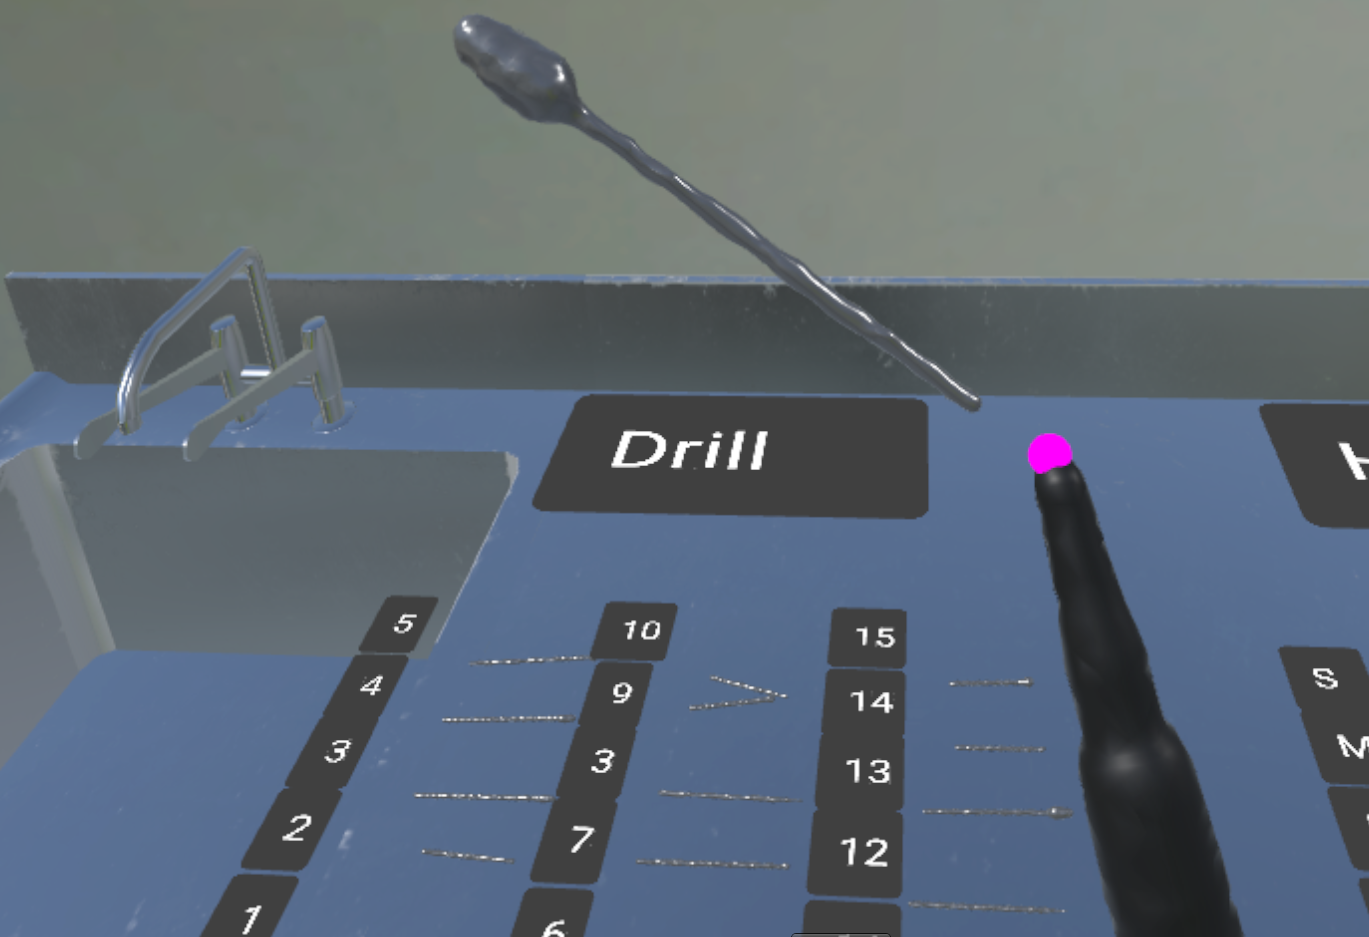
\includegraphics[width=200px]{images/implementation/features/procedures/drilling_attachment.png}
    \caption{\label{fig::FeatureDrillingAttachments}Process of attaching drill bit to the drill handle. With the right hand, the user performs the indicate action by touching 
    the respective button. With the other hand, the bit is picked up by grabbing it and moved into the pink sphere to attach the attachment.}
\end{figure}

In total, there are fifteen bits which can be used as an attachment for the drilling procedure.
Bits are modeled after their real counterparts in UHA.
They differ in size, length and width.
A visual signal is shown to the user while the indicate action is performed on the hand holding the drill handle.
By moving a drill bit to the visual indicator, the bit is attached to the handle (Figure \ref{fig::FeatureDrillingAttachments}).
Swapping out bits is performed by simply moving another bit into the indicator.
To perform the procedure, the drill handle must have a bit attached. 

\begin{figure}[ht]
    \centering
    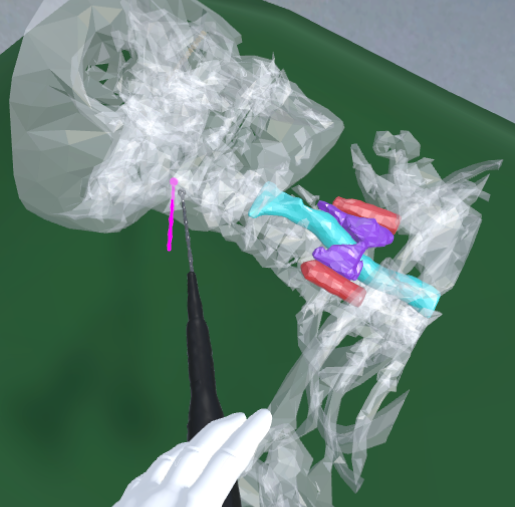
\includegraphics[width=200px]{images/implementation/features/procedures/drilling.png}
    \caption{\label{fig::FeatureDrilling}Drilling procedure. The pink object represents the last performed step, which was performed using the currently selected tool by pressing 
    the respective button all the way.}
\end{figure}

By triggering the perform action of the hand holding the drill, a copy of the currently attached drill bit is created and added to the project case. 
This copy has a different material, i.e. a pink material, to indicate that it is part of the project case (Figure \ref{fig::FeatureDrilling}).
Additionally, textual information about the currently attached drill bit will be stored in the project case, so that the exact procedure can be reproduced later (Requirements \ref{req::N3}, \ref{req::N5}).
The drill bit will not be removed on performing a procedure, so that multiple drilling steps can be performed consecutively.
When the drill is no longer needed, it can either be placed back on the instrument tray or the operating table for quick access.
Note that any instrument, excluding the osteosynthesis plates described later, can be placed anywhere in the OT.
\paragraph{Chiseling}

The \textbf{chiseling} procedure has two parts to it.
First, with one hand a chisel has to be chosen.
Users have a choice between a small, medium, large and extra large chisel to perform the procedure.
With the other hand, users then have to pick up the hammer.
Since this procedure requires users to hold two surgical instruments at the same time, this procedure can get cumbersome.
However, users can easily avoid this by placing the instruments on the operating table in the middle of the OT and repositioning afterwards (Figure \ref{fig::ChiselPrepare}).

\begin{figure}[ht]
    \centering
    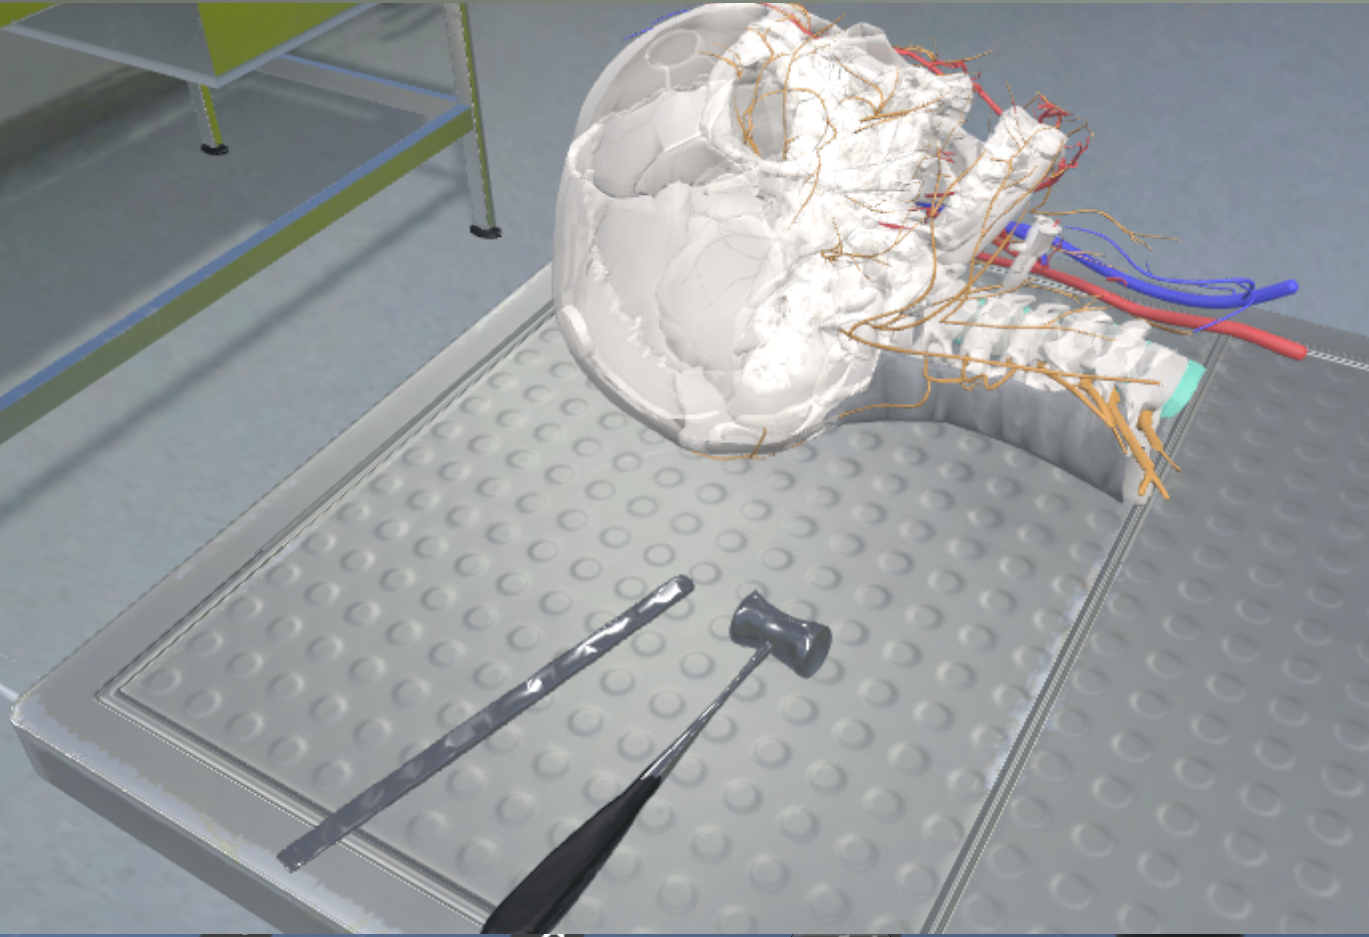
\includegraphics[width=\linewidth]{images/implementation/features/procedures/chisel_prepare.png}
    \caption{\label{fig::ChiselPrepare}The user prepares for the chiseling procedure by placing the instruments on the OT where the patient is located.
    indicators with the hammer in the other hand to perform the procedure.}
\end{figure}

When users have the perfect viewpoint, they can take up both instruments once again and start the procedure.
By pressing the indicate button on the hand where the chisel is located, rectangular indications at the top and bottom end of the chisel are shown to the user.
While these indications are active, the user has to perform a hammering motion with the hand holding the hammer.

\begin{figure}[ht]
    \centering
    \begin{minipage}{.5\textwidth}
      \centering
      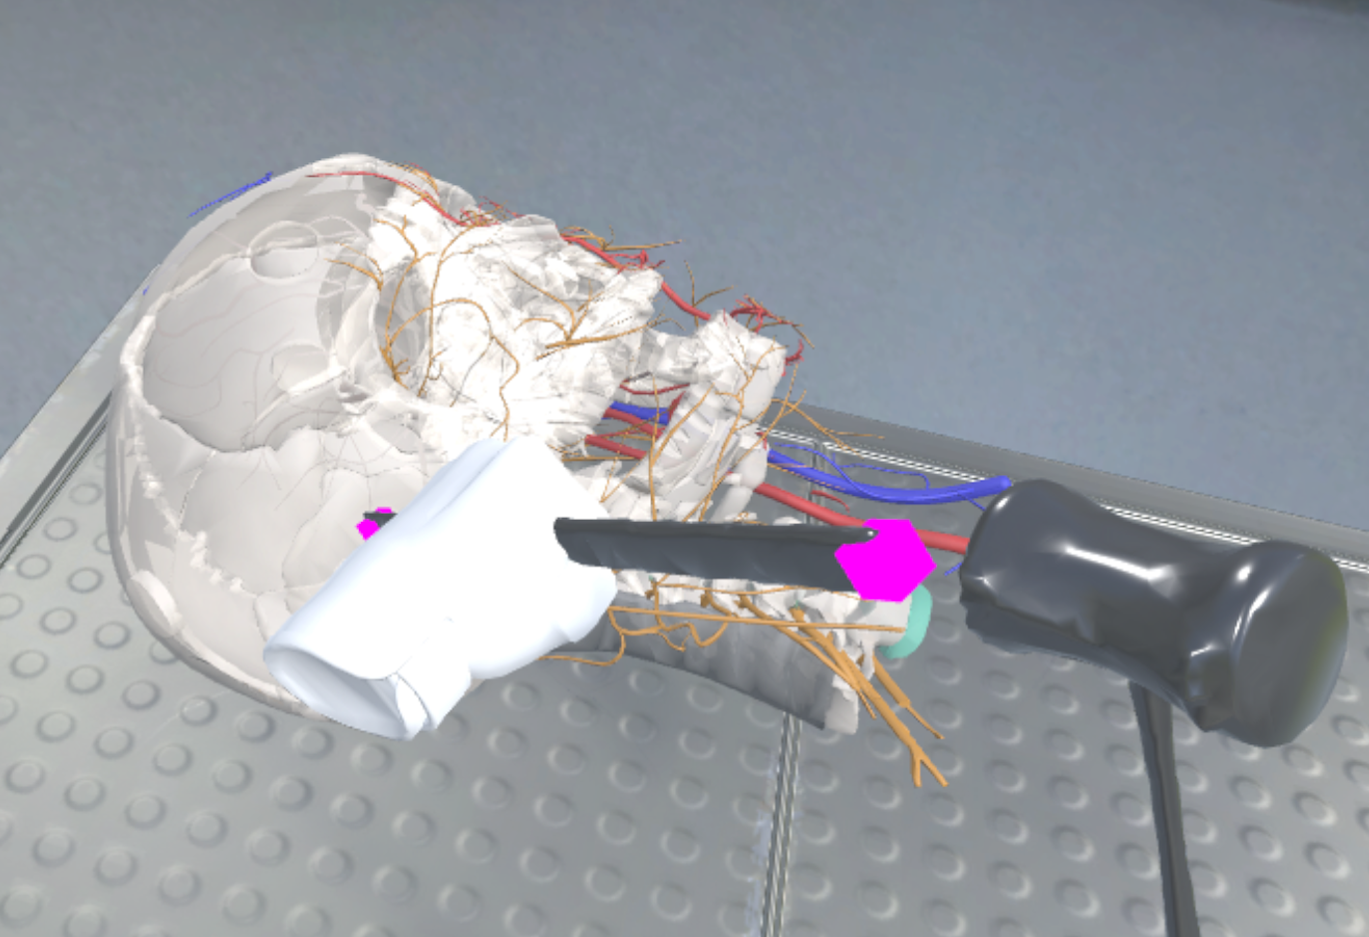
\includegraphics[width=0.99\linewidth]{images/implementation/features/procedures/chisel_1.png}
    \end{minipage}%
    \begin{minipage}{.5\textwidth}
      \centering
      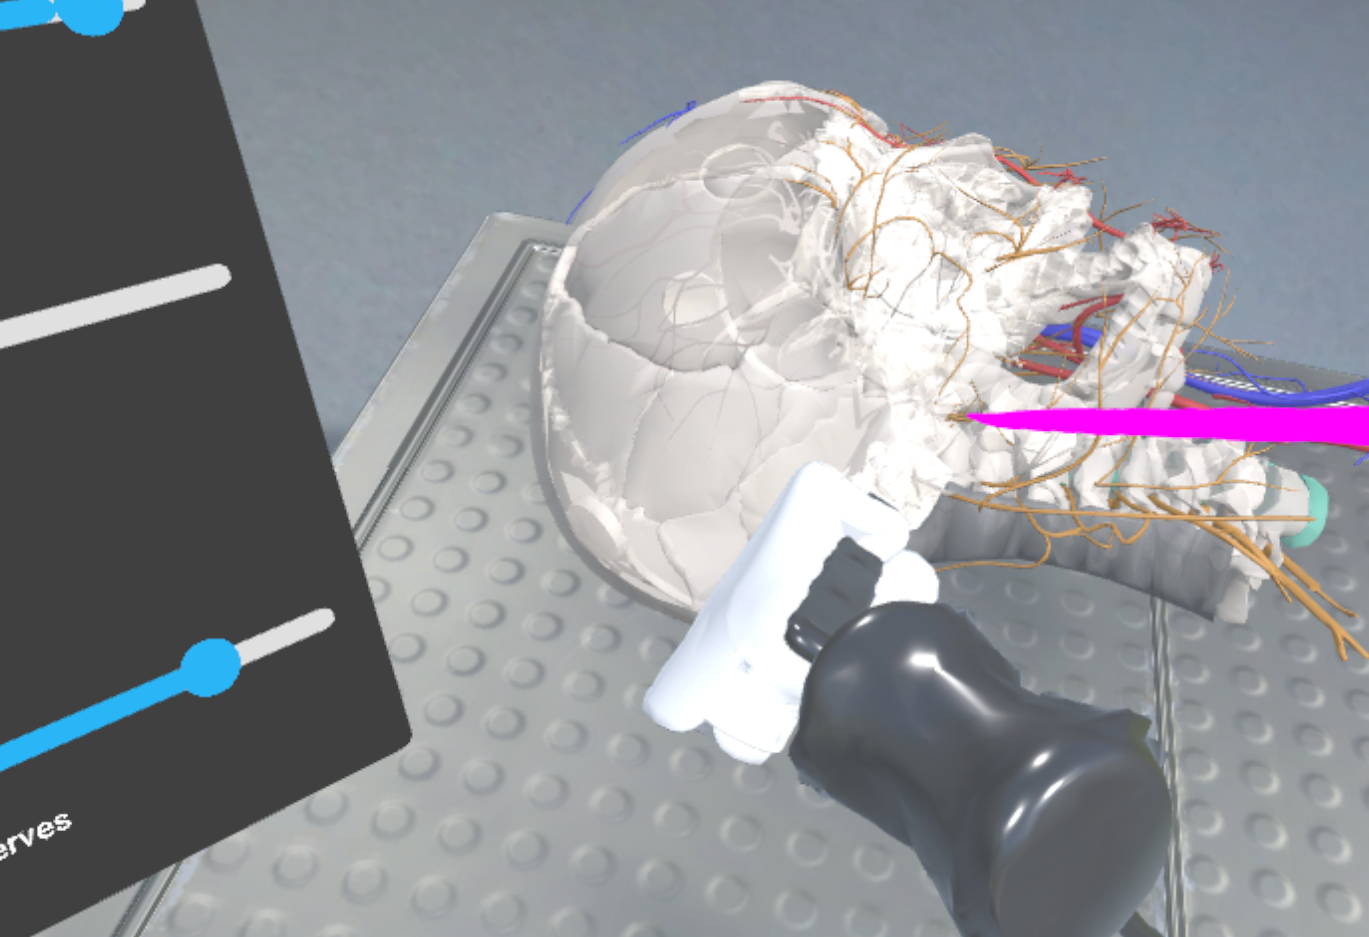
\includegraphics[width=0.99\linewidth]{images/implementation/features/procedures/chisel_2.png}
    \end{minipage}
    \caption{\label{fig::ChiselProcedure}Process of the chiseling procedure. Left: The users uses the indicate action with his left hand in preparation for the procedure. Right: After hammering on the indication on the chisel, the procedure has been performed and a step is generated.}
\end{figure}

When they hit the rectangular indicators located on the chisel, the chiseling procedure step is added to the project case in form of a modified copy of the hold chisel (Figure \ref{fig::ChiselProcedure}).
Here, information about the performed step is also included in the form of chisel size used for the procedure. 
\paragraph{Sawing}

\begin{figure}[ht]
    \centering
    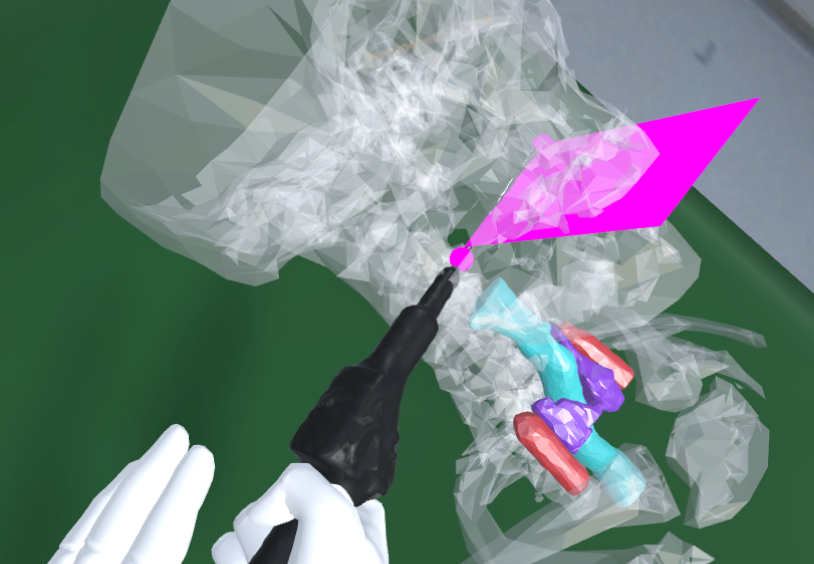
\includegraphics[width=200px]{images/implementation/features/procedures/bonesaw.png}
    \caption{\label{fig::FeatureBoneSaw}Bonesaw Procedure}
\end{figure}

The \textbf{sawing} procedure is performed by picking up the bonesaw.
Touch the controller will show two indications to the user (Figure \ref{fig::FeatureBoneSaw}).
The procedure is performed by first pressing down the trigger button and then letting go of it.
When letting go of the trigger button, a two dimensianal plane is created in the three dimensional space by using four points.
Two of these points are created when pressing down, and the other two when letting go of the trigger button.
A plane is then created with which the user can reproduce the way in which the bonesaw has been moved.
Arbitrary cutting shapes can be created by breaking them down into two-dimensional shapes and performing multiple movements.
\paragraph{Milling}

\begin{figure}[ht]
    \centering
    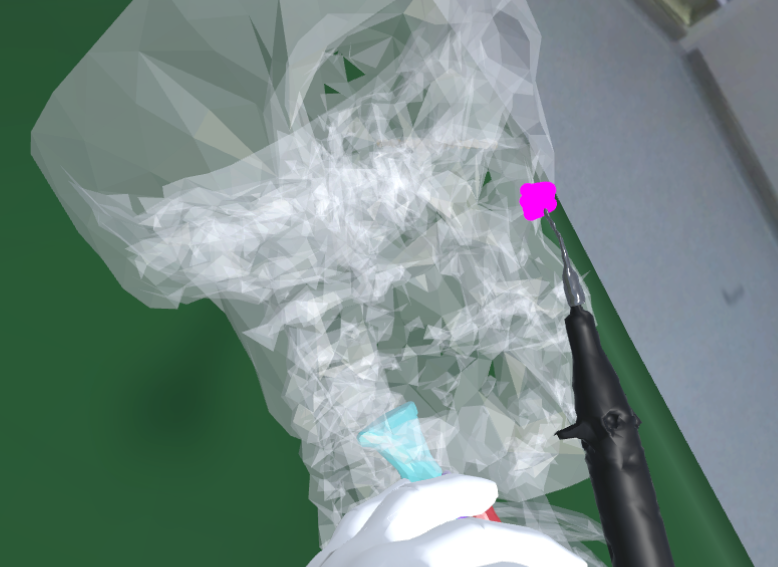
\includegraphics[width=200px]{images/implementation/features/procedures/piezo.png}
    \caption{\label{fig::FeaturePiezo}Milling procedure. Holding down the trigger button will draw little spheres until the button is released. The resulting object represents the volumetric space which is to be milled.}
\end{figure}

The \textbf{milling} operation is performed by grabbing the piezo instrument.
The indicator for the piezo is at the tip of the instrument, indicating which area will be milled.
While the "perform" button is being held down, little spheres are being drawn at the tip of the instrument \ref{fig::FeaturePiezo}.
When the button is released, the shapes are combined into a single 3D model and added as a project step.
The resulting object represents the volumetric space which has to be milled in the procedure.
The procedure can be reconstructed by "milling" the same 3D space in the virtual operating room.
\begin{figure}[ht!]
    \centering
    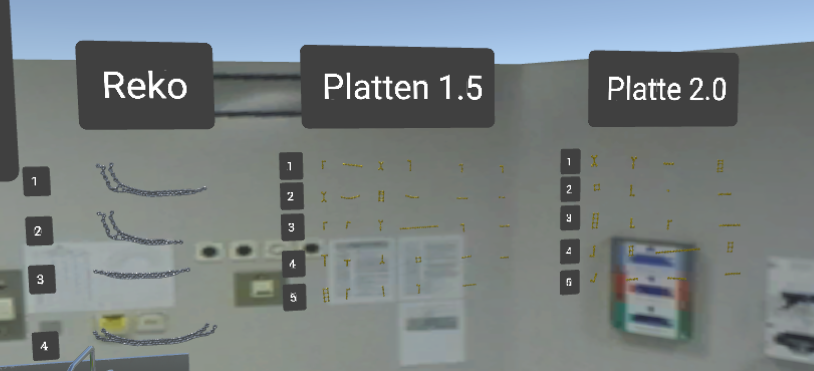
\includegraphics[width=\linewidth]{images/implementation/features/procedures/metal_plates_1.png}
    \caption{\label{fig::FeatureMetalPlate} Osteosynthesis Plates Overview}
\end{figure}

The osteosynthesis plates procedure consists of two steps before adding it as a step to the project case.
First, users have to chose which plate to use (Figure \ref{fig::FeatureMetalPlate}).
The user can chose from four reconstruction plates, 29 1.5mm plates and 20 2.0mm plates (Firma Angeben, osteosynthesis plates).
The optimal plates to use vary due to the pathology of the patient and the previously performed procedures.
After selecting the proper plate, a number of indicators will show to the user (Figure \ref{fig::FeatureMetalPlate2}).
In the context of the osteosynthesis plates, these indicators are "control points", with which the user can bend and twist the plates.
Bending and twisting is performed by chosing a control point via hovering them with the users free hand and grabbing them.
Then, the user has to translate and rotate the control point in the desired manner.
\begin{figure}
  \centering
  \begin{minipage}{.5\textwidth}
    \centering
    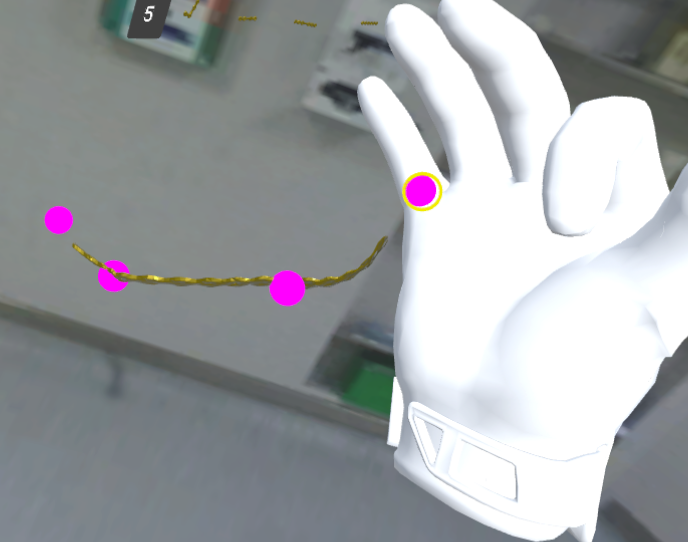
\includegraphics[width=0.95\linewidth]{images/implementation/features/procedures/metal_plates_2.png}
  \end{minipage}%
  \begin{minipage}{.5\textwidth}
    \centering
    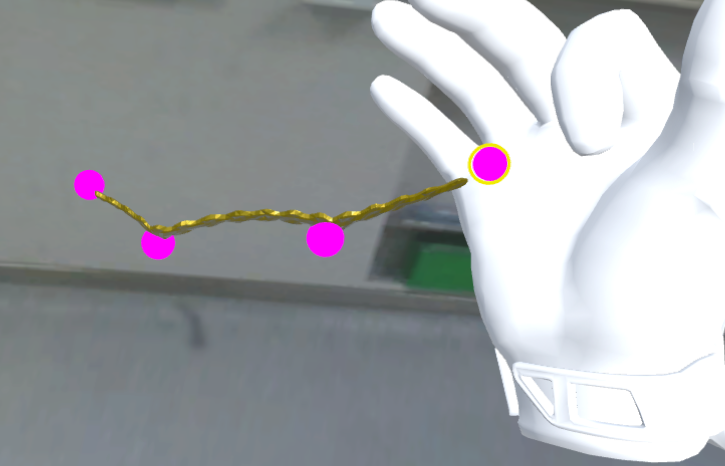
\includegraphics[width=0.95\linewidth]{images/implementation/features/procedures/metal_plates_3.png}
  \end{minipage}
  \caption{\label{fig::FeatureMetalPlate2}Osteosynthesis Plates Modifications. User can translate and rotate "control points" to perform modifications to the plates shape} 
\end{figure}

The user can then observe in which way this has affected the shape of the metal plate and either position the plate on the patient or perform more modifications to the plates via controlpoints.
The correct modification of the metal plates differs quite a lot from real life modifications to the plates.
However even though there is a slight learning curve to it, the modification is consistent and predictable (Figure \ref{fig::FeatureMetalPlate2}).


\begin{figure}[ht!]
    \centering
    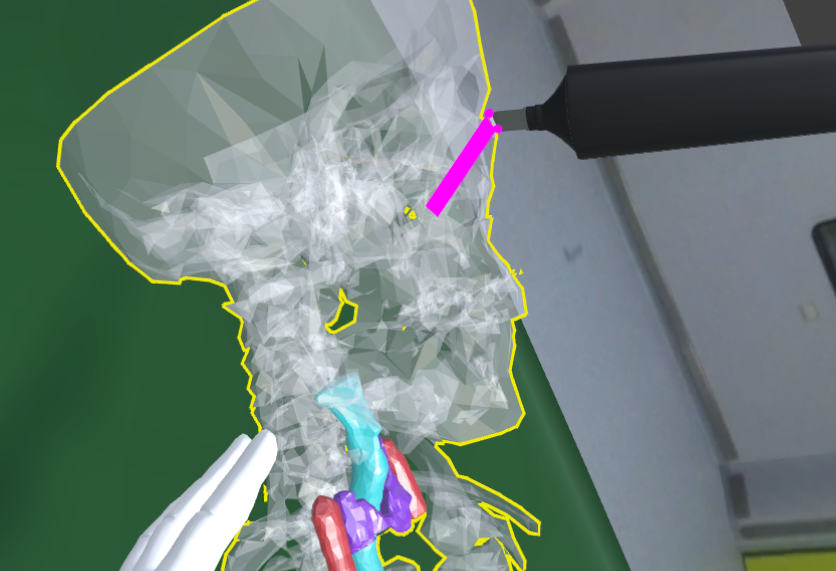
\includegraphics[width=\linewidth]{images/implementation/features/procedures/marker.png}
    \caption{\label{fig::FeatureMarker}Marker Procedure}
\end{figure}

The marking procedure is similar to the bonesaw procedure, meaning that rectangular shapes are drawed into the three dimensianal space (Figure \ref{fig::FeatureMarker}).
However, here the created shapes are much thinner.
In contrast to the bonesaw, the virtual hands of the user are also disabled here.
This way, the user can decide to hold the marker in the optimal way.
Since the main objective is marking specific spots on the patient, this is the natural approach.

\chapter{\label{chap::RelatedWork}Related Work}
At this point, the aforementioned six procedures are implemented in the system.
However, as described in Section \ref{sec::Architecture}, the system is extensible in the regard that new instruments can be implemented.
Currently, the implemented instruments are based on the workflow of OMF surgeons of the UHA: Users can perform drilling, hammer and chisel, bonesaw and milling operations.
Additionally, users can place markings and osteosynthesis plates on the virtual patient.
\\ To perform procedures, a project case has to be loaded first, as described in Section \ref{sec::GraphicalUserInterface}.
In the sense of SteamVRs interaction system described in Section \ref{sec::Architecture}, for each procedure there is an 'indicate' action when the user touches the 'perform' button, as well as an 'perform' action when the user presses the button all the way.
This way, users get a visual feedback when they are about to perform a procedure, as well as having visual indications of where the procedure will start (i.e. tip of the surgical instrument).
After described each procedure individually, how the procedures come together to create the steps for a procedure will be shortly desctribed.
\\ Each procedure will add a step to the project case.
In the sense of the VR-AR-based workflow described in Section \ref{sec::Workflow}, project cases can then be loaded into both parts of the workflow.
The steps are added to the hierarchy of the patient's 3D model and are identified as a step by name.
Through using this kind of approach, extensibility is guaranteed as each new instrument simply has to add some kind of geometry as a step to the project case (Requirements \ref{req::N8}, \ref{req::F3.7}).
It follows that any kind of procedure can then be imported into the AR workflow, even without touching the application.
\\ When a procedure is performed, users get voice feedback confirming that a step has been added to the project case.
Users can also navigate the project cases steps by using the VUIs commands, so that navigation through the steps of the procedure can be done while holding surgical instruments (Requirements \ref{req::N1}, \ref{req::F3.7}).
\\ For some of the surgical instruments, the user representation of the hand will be shown, for others not.
When a surgical instrument has this feature implemented, it is guaranteed that the instrument will always be grabbed and positioned in the same position on the hand, meaning the handgrip will always be the same.
However, in some cases, f.e. sawing with the bonesaw, this feature would prevent users from switching the handgrip of the surgical instrument. 
Therefore, for some instruments, this feature was removed.
Users will not see their virtual hands on the surgical instrument, but can chose to hold it however they want.
The virtual hands will be hidden while holding the instrument, however the instrument still represents the users hand position.
This way, the handgrip of the instrument can be adapted as users see fit.
The decision, on which was decided if hands should be hidden when grabbing an instrument, was made by a trial and error approach with the help of a physician's opinion on whether this features was useful.
The procedure specific implementation will be thoroughly described in the following.

\paragraph{Drilling}

The \textbf{drilling} operation is performed by first picking up the drill handle from the instrument tray via the grabbing action (Figure \ref{fig::FeatureDrillingAttachments}).
Since drills are typically held in a number of different ways, the handgrip of the drill handle is adjustable.
Therefore, the virtual hand will not be displayed while holding the drill.
The instrument tray is located next to the operating table, where the patient's model will initially be positioned.
The drill handle initially has no attachment; users have to attach a drill bit first.

\begin{figure}[ht]
    \centering
    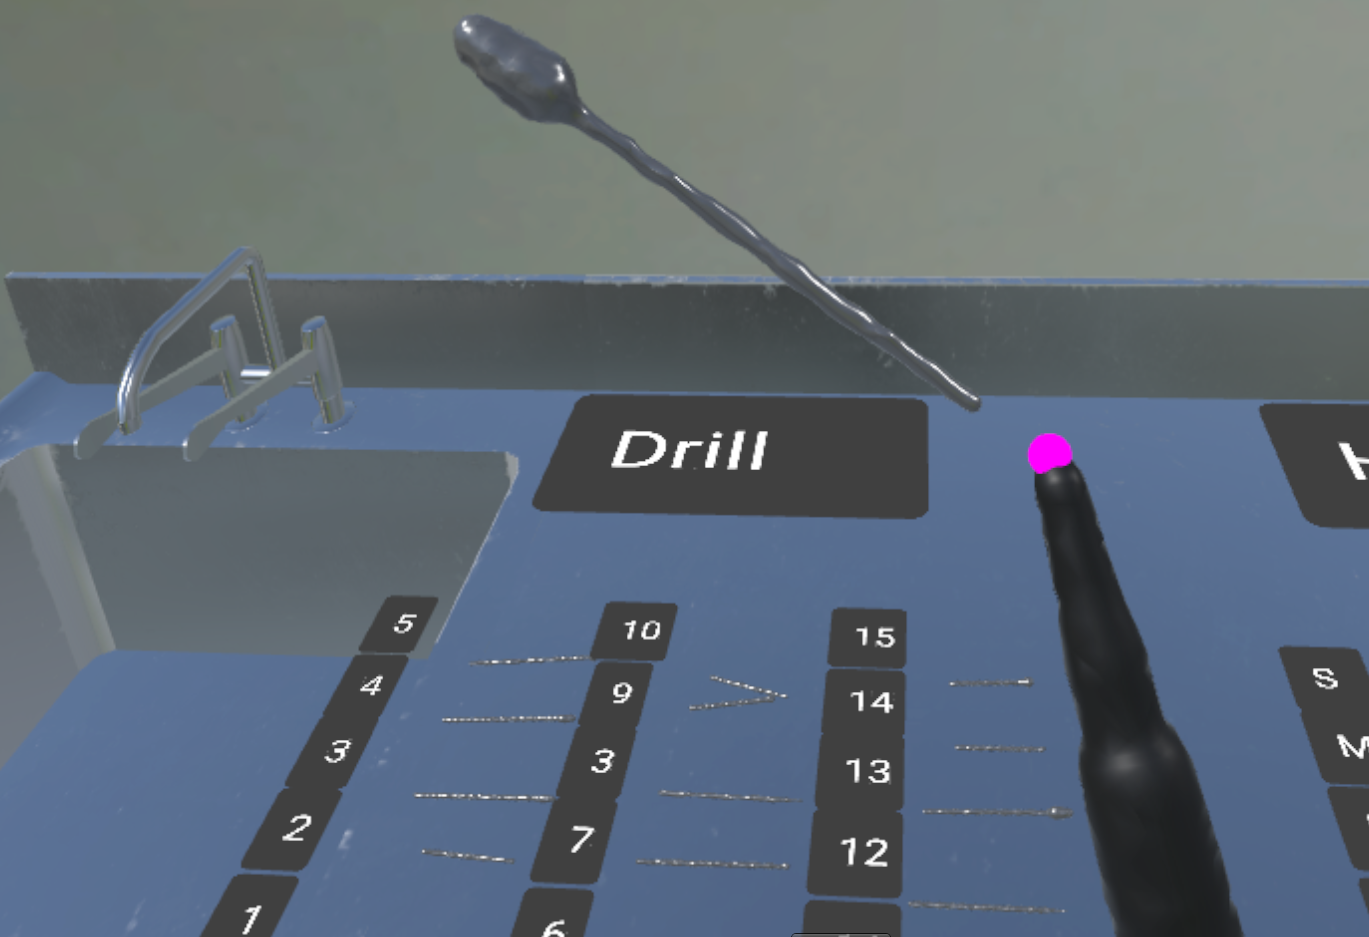
\includegraphics[width=200px]{images/implementation/features/procedures/drilling_attachment.png}
    \caption{\label{fig::FeatureDrillingAttachments}Process of attaching drill bit to the drill handle. With the right hand, the user performs the indicate action by touching 
    the respective button. With the other hand, the bit is picked up by grabbing it and moved into the pink sphere to attach the attachment.}
\end{figure}

In total, there are fifteen bits which can be used as an attachment for the drilling procedure.
Bits are modeled after their real counterparts in UHA.
They differ in size, length and width.
A visual signal is shown to the user while the indicate action is performed on the hand holding the drill handle.
By moving a drill bit to the visual indicator, the bit is attached to the handle (Figure \ref{fig::FeatureDrillingAttachments}).
Swapping out bits is performed by simply moving another bit into the indicator.
To perform the procedure, the drill handle must have a bit attached. 

\begin{figure}[ht]
    \centering
    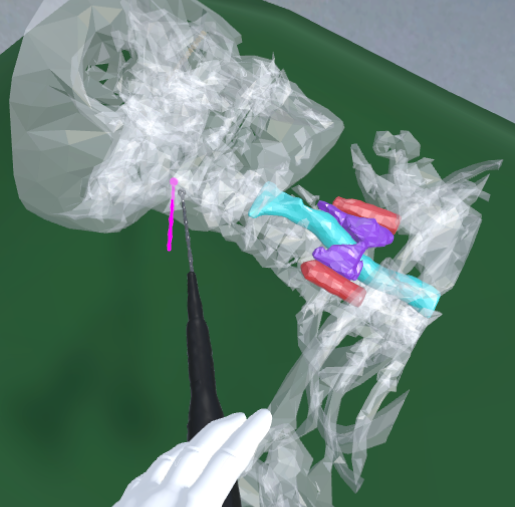
\includegraphics[width=200px]{images/implementation/features/procedures/drilling.png}
    \caption{\label{fig::FeatureDrilling}Drilling procedure. The pink object represents the last performed step, which was performed using the currently selected tool by pressing 
    the respective button all the way.}
\end{figure}

By triggering the perform action of the hand holding the drill, a copy of the currently attached drill bit is created and added to the project case. 
This copy has a different material, i.e. a pink material, to indicate that it is part of the project case (Figure \ref{fig::FeatureDrilling}).
Additionally, textual information about the currently attached drill bit will be stored in the project case, so that the exact procedure can be reproduced later (Requirements \ref{req::N3}, \ref{req::N5}).
The drill bit will not be removed on performing a procedure, so that multiple drilling steps can be performed consecutively.
When the drill is no longer needed, it can either be placed back on the instrument tray or the operating table for quick access.
Note that any instrument, excluding the osteosynthesis plates described later, can be placed anywhere in the OT.
\paragraph{Chiseling}

The \textbf{chiseling} procedure has two parts to it.
First, with one hand a chisel has to be chosen.
Users have a choice between a small, medium, large and extra large chisel to perform the procedure.
With the other hand, users then have to pick up the hammer.
Since this procedure requires users to hold two surgical instruments at the same time, this procedure can get cumbersome.
However, users can easily avoid this by placing the instruments on the operating table in the middle of the OT and repositioning afterwards (Figure \ref{fig::ChiselPrepare}).

\begin{figure}[ht]
    \centering
    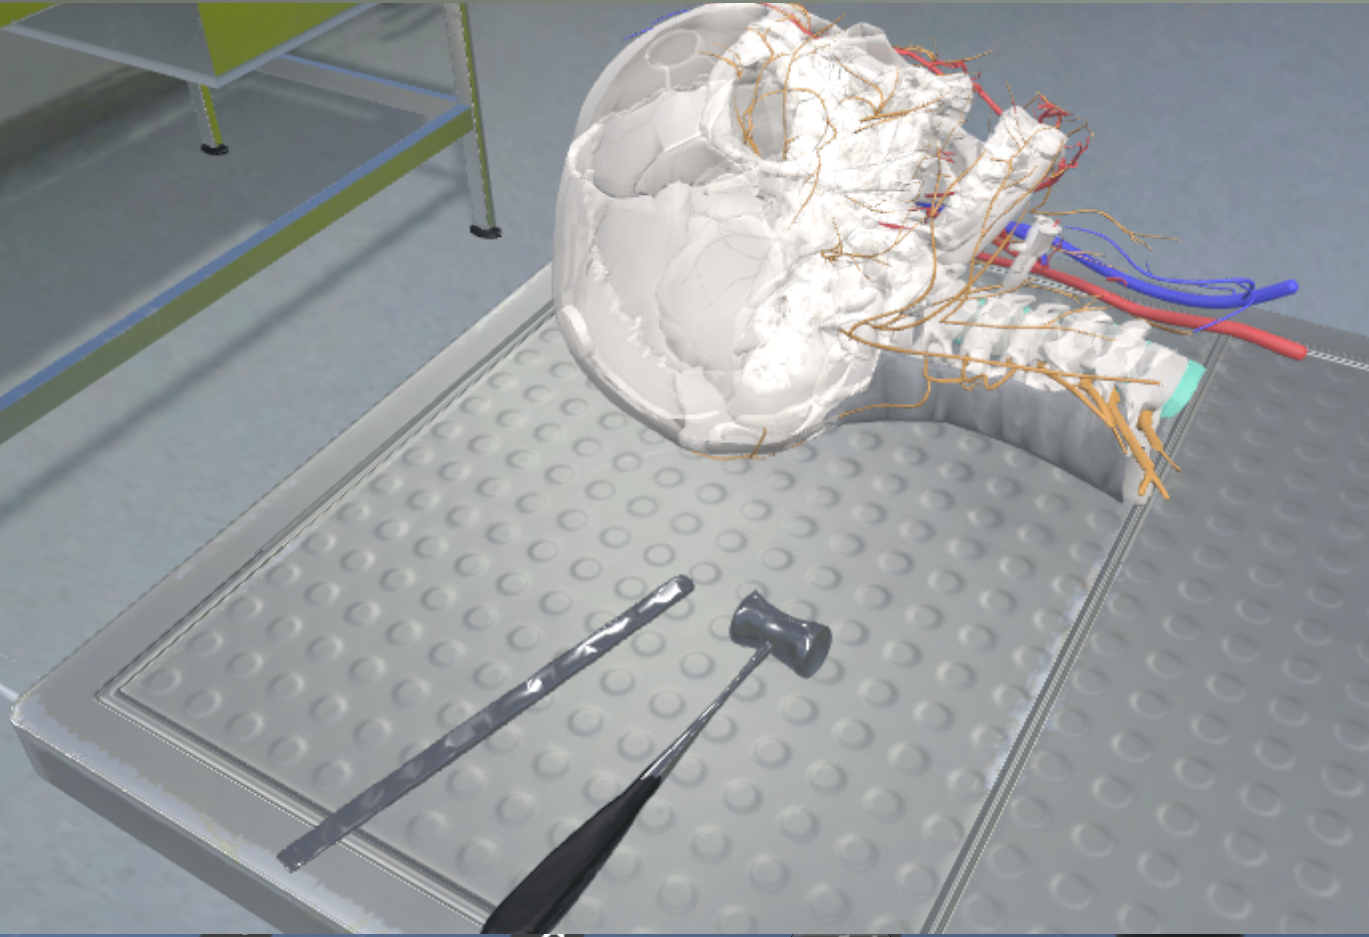
\includegraphics[width=\linewidth]{images/implementation/features/procedures/chisel_prepare.png}
    \caption{\label{fig::ChiselPrepare}The user prepares for the chiseling procedure by placing the instruments on the OT where the patient is located.
    indicators with the hammer in the other hand to perform the procedure.}
\end{figure}

When users have the perfect viewpoint, they can take up both instruments once again and start the procedure.
By pressing the indicate button on the hand where the chisel is located, rectangular indications at the top and bottom end of the chisel are shown to the user.
While these indications are active, the user has to perform a hammering motion with the hand holding the hammer.

\begin{figure}[ht]
    \centering
    \begin{minipage}{.5\textwidth}
      \centering
      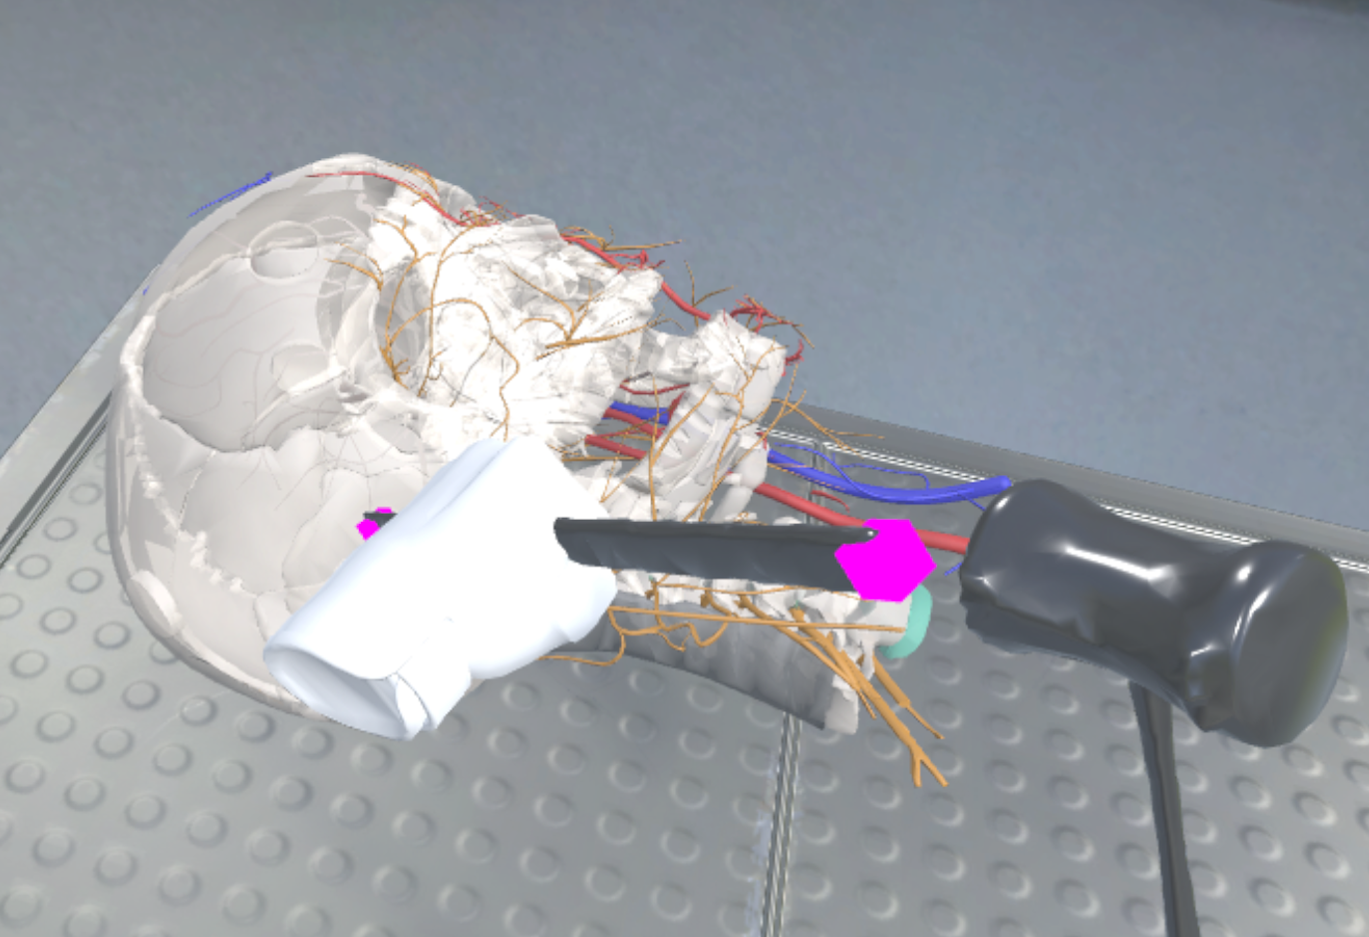
\includegraphics[width=0.99\linewidth]{images/implementation/features/procedures/chisel_1.png}
    \end{minipage}%
    \begin{minipage}{.5\textwidth}
      \centering
      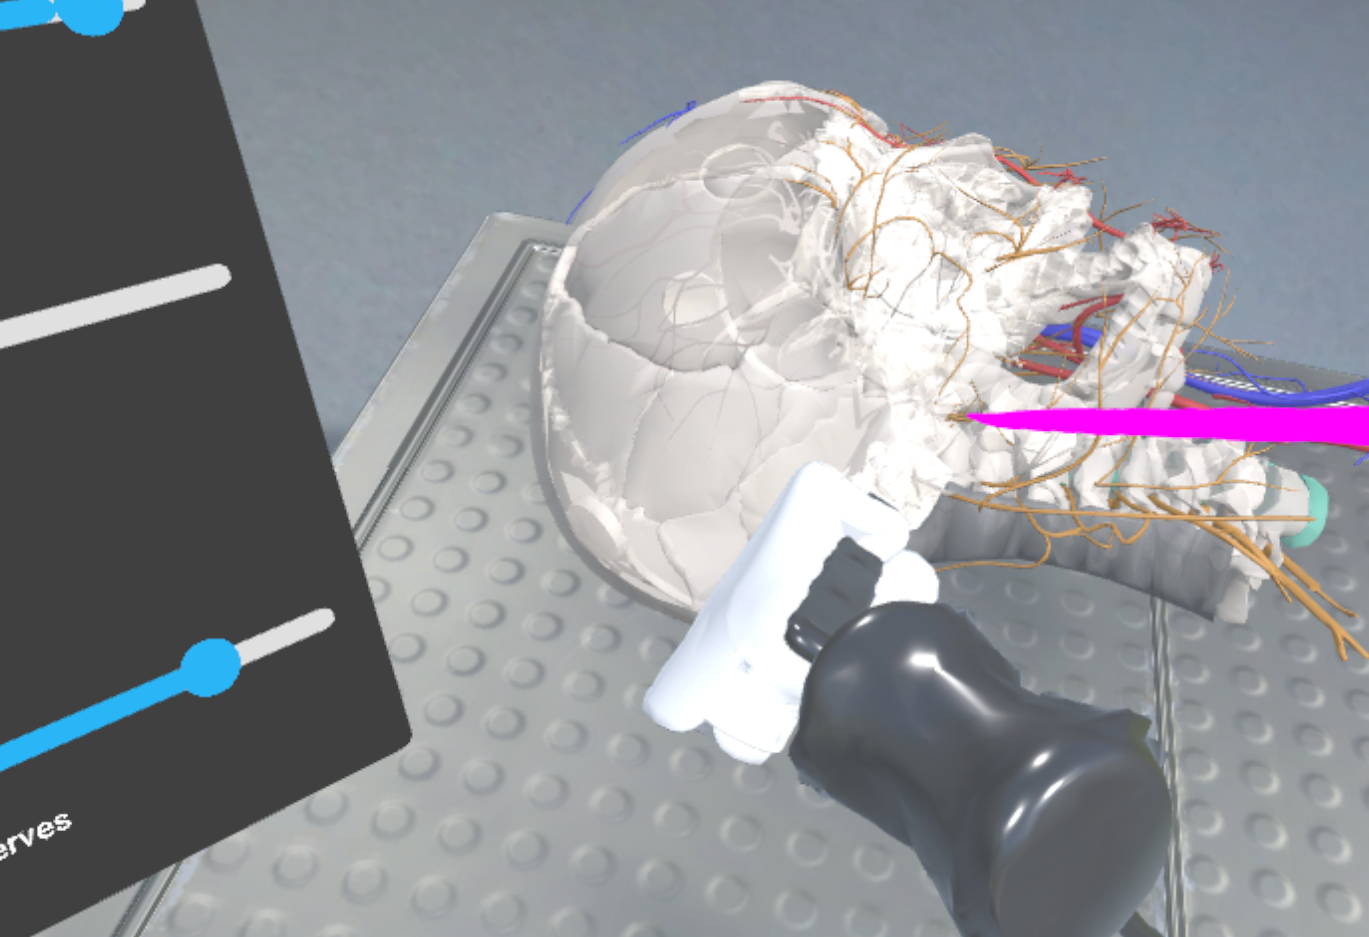
\includegraphics[width=0.99\linewidth]{images/implementation/features/procedures/chisel_2.png}
    \end{minipage}
    \caption{\label{fig::ChiselProcedure}Process of the chiseling procedure. Left: The users uses the indicate action with his left hand in preparation for the procedure. Right: After hammering on the indication on the chisel, the procedure has been performed and a step is generated.}
\end{figure}

When they hit the rectangular indicators located on the chisel, the chiseling procedure step is added to the project case in form of a modified copy of the hold chisel (Figure \ref{fig::ChiselProcedure}).
Here, information about the performed step is also included in the form of chisel size used for the procedure. 
\paragraph{Sawing}

\begin{figure}[ht]
    \centering
    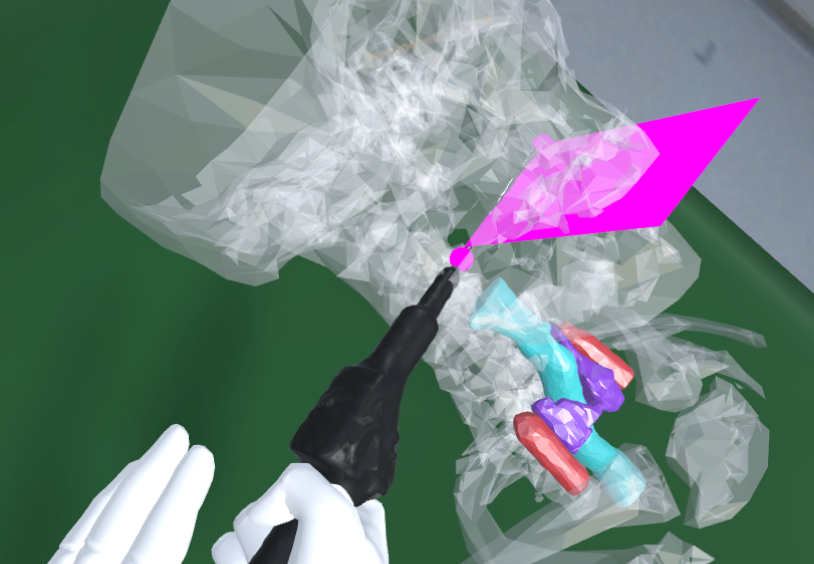
\includegraphics[width=200px]{images/implementation/features/procedures/bonesaw.png}
    \caption{\label{fig::FeatureBoneSaw}Bonesaw Procedure}
\end{figure}

The \textbf{sawing} procedure is performed by picking up the bonesaw.
Touch the controller will show two indications to the user (Figure \ref{fig::FeatureBoneSaw}).
The procedure is performed by first pressing down the trigger button and then letting go of it.
When letting go of the trigger button, a two dimensianal plane is created in the three dimensional space by using four points.
Two of these points are created when pressing down, and the other two when letting go of the trigger button.
A plane is then created with which the user can reproduce the way in which the bonesaw has been moved.
Arbitrary cutting shapes can be created by breaking them down into two-dimensional shapes and performing multiple movements.
\paragraph{Milling}

\begin{figure}[ht]
    \centering
    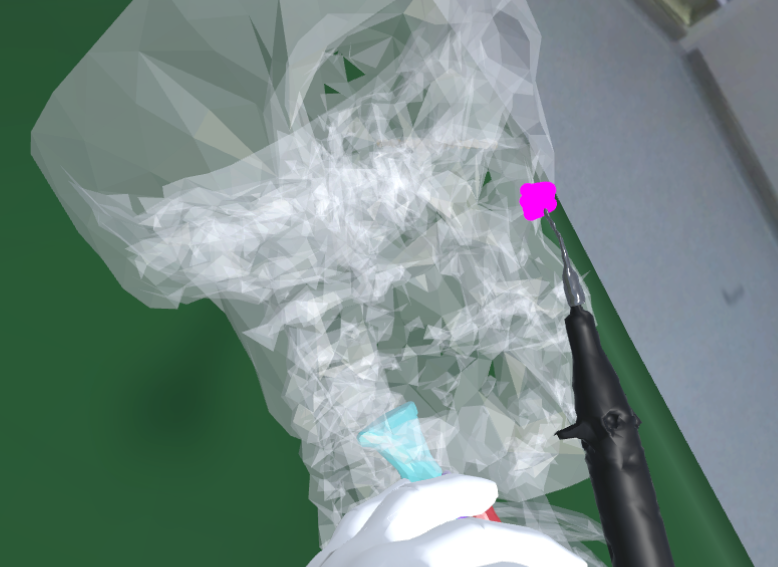
\includegraphics[width=200px]{images/implementation/features/procedures/piezo.png}
    \caption{\label{fig::FeaturePiezo}Milling procedure. Holding down the trigger button will draw little spheres until the button is released. The resulting object represents the volumetric space which is to be milled.}
\end{figure}

The \textbf{milling} operation is performed by grabbing the piezo instrument.
The indicator for the piezo is at the tip of the instrument, indicating which area will be milled.
While the "perform" button is being held down, little spheres are being drawn at the tip of the instrument \ref{fig::FeaturePiezo}.
When the button is released, the shapes are combined into a single 3D model and added as a project step.
The resulting object represents the volumetric space which has to be milled in the procedure.
The procedure can be reconstructed by "milling" the same 3D space in the virtual operating room.
\begin{figure}[ht!]
    \centering
    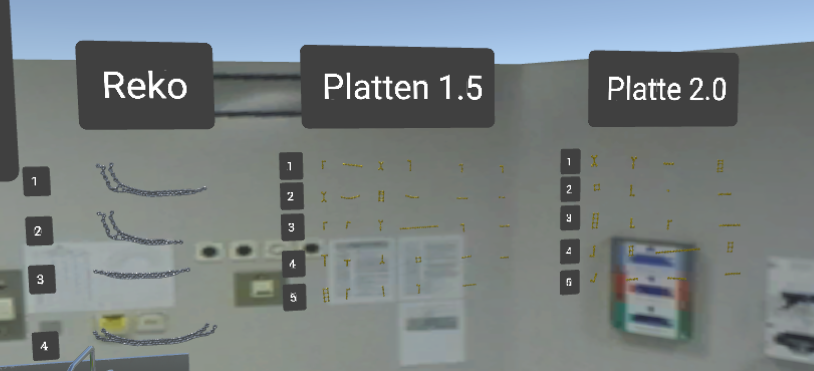
\includegraphics[width=\linewidth]{images/implementation/features/procedures/metal_plates_1.png}
    \caption{\label{fig::FeatureMetalPlate} Osteosynthesis Plates Overview}
\end{figure}

The osteosynthesis plates procedure consists of two steps before adding it as a step to the project case.
First, users have to chose which plate to use (Figure \ref{fig::FeatureMetalPlate}).
The user can chose from four reconstruction plates, 29 1.5mm plates and 20 2.0mm plates (Firma Angeben, osteosynthesis plates).
The optimal plates to use vary due to the pathology of the patient and the previously performed procedures.
After selecting the proper plate, a number of indicators will show to the user (Figure \ref{fig::FeatureMetalPlate2}).
In the context of the osteosynthesis plates, these indicators are "control points", with which the user can bend and twist the plates.
Bending and twisting is performed by chosing a control point via hovering them with the users free hand and grabbing them.
Then, the user has to translate and rotate the control point in the desired manner.
\begin{figure}
  \centering
  \begin{minipage}{.5\textwidth}
    \centering
    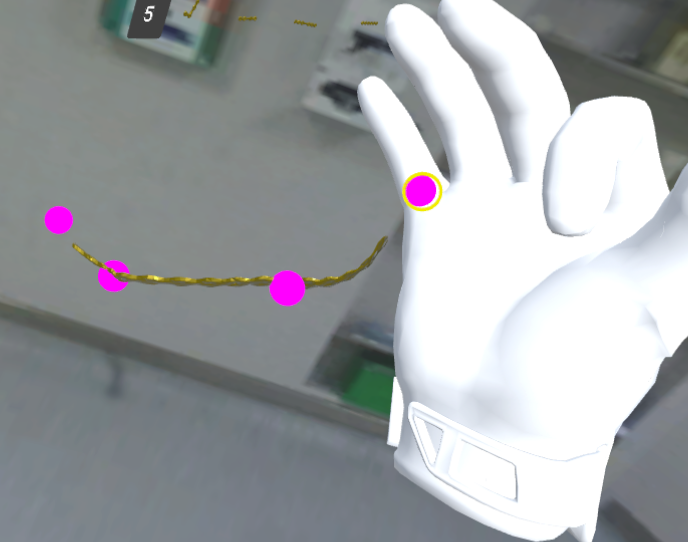
\includegraphics[width=0.95\linewidth]{images/implementation/features/procedures/metal_plates_2.png}
  \end{minipage}%
  \begin{minipage}{.5\textwidth}
    \centering
    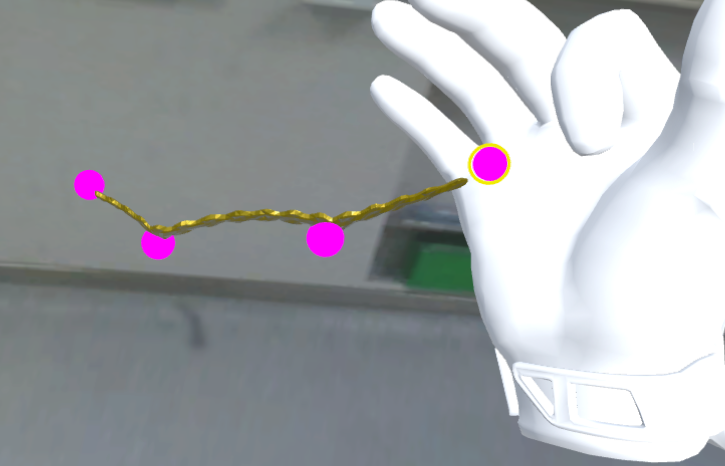
\includegraphics[width=0.95\linewidth]{images/implementation/features/procedures/metal_plates_3.png}
  \end{minipage}
  \caption{\label{fig::FeatureMetalPlate2}Osteosynthesis Plates Modifications. User can translate and rotate "control points" to perform modifications to the plates shape} 
\end{figure}

The user can then observe in which way this has affected the shape of the metal plate and either position the plate on the patient or perform more modifications to the plates via controlpoints.
The correct modification of the metal plates differs quite a lot from real life modifications to the plates.
However even though there is a slight learning curve to it, the modification is consistent and predictable (Figure \ref{fig::FeatureMetalPlate2}).


\begin{figure}[ht!]
    \centering
    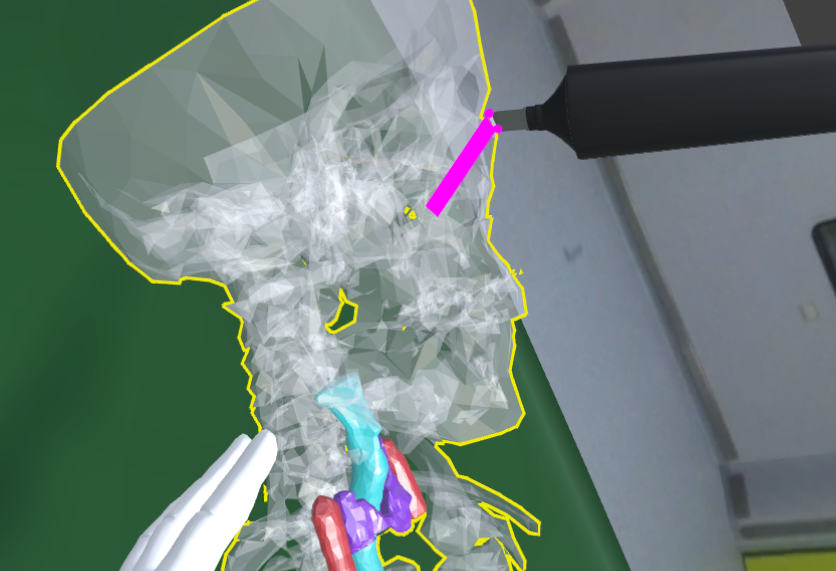
\includegraphics[width=\linewidth]{images/implementation/features/procedures/marker.png}
    \caption{\label{fig::FeatureMarker}Marker Procedure}
\end{figure}

The marking procedure is similar to the bonesaw procedure, meaning that rectangular shapes are drawed into the three dimensianal space (Figure \ref{fig::FeatureMarker}).
However, here the created shapes are much thinner.
In contrast to the bonesaw, the virtual hands of the user are also disabled here.
This way, the user can decide to hold the marker in the optimal way.
Since the main objective is marking specific spots on the patient, this is the natural approach.

\chapter{\label{chap::Approach}Approach}
At this point, the aforementioned six procedures are implemented in the system.
However, as described in Section \ref{sec::Architecture}, the system is extensible in the regard that new instruments can be implemented.
Currently, the implemented instruments are based on the workflow of OMF surgeons of the UHA: Users can perform drilling, hammer and chisel, bonesaw and milling operations.
Additionally, users can place markings and osteosynthesis plates on the virtual patient.
\\ To perform procedures, a project case has to be loaded first, as described in Section \ref{sec::GraphicalUserInterface}.
In the sense of SteamVRs interaction system described in Section \ref{sec::Architecture}, for each procedure there is an 'indicate' action when the user touches the 'perform' button, as well as an 'perform' action when the user presses the button all the way.
This way, users get a visual feedback when they are about to perform a procedure, as well as having visual indications of where the procedure will start (i.e. tip of the surgical instrument).
After described each procedure individually, how the procedures come together to create the steps for a procedure will be shortly desctribed.
\\ Each procedure will add a step to the project case.
In the sense of the VR-AR-based workflow described in Section \ref{sec::Workflow}, project cases can then be loaded into both parts of the workflow.
The steps are added to the hierarchy of the patient's 3D model and are identified as a step by name.
Through using this kind of approach, extensibility is guaranteed as each new instrument simply has to add some kind of geometry as a step to the project case (Requirements \ref{req::N8}, \ref{req::F3.7}).
It follows that any kind of procedure can then be imported into the AR workflow, even without touching the application.
\\ When a procedure is performed, users get voice feedback confirming that a step has been added to the project case.
Users can also navigate the project cases steps by using the VUIs commands, so that navigation through the steps of the procedure can be done while holding surgical instruments (Requirements \ref{req::N1}, \ref{req::F3.7}).
\\ For some of the surgical instruments, the user representation of the hand will be shown, for others not.
When a surgical instrument has this feature implemented, it is guaranteed that the instrument will always be grabbed and positioned in the same position on the hand, meaning the handgrip will always be the same.
However, in some cases, f.e. sawing with the bonesaw, this feature would prevent users from switching the handgrip of the surgical instrument. 
Therefore, for some instruments, this feature was removed.
Users will not see their virtual hands on the surgical instrument, but can chose to hold it however they want.
The virtual hands will be hidden while holding the instrument, however the instrument still represents the users hand position.
This way, the handgrip of the instrument can be adapted as users see fit.
The decision, on which was decided if hands should be hidden when grabbing an instrument, was made by a trial and error approach with the help of a physician's opinion on whether this features was useful.
The procedure specific implementation will be thoroughly described in the following.

\paragraph{Drilling}

The \textbf{drilling} operation is performed by first picking up the drill handle from the instrument tray via the grabbing action (Figure \ref{fig::FeatureDrillingAttachments}).
Since drills are typically held in a number of different ways, the handgrip of the drill handle is adjustable.
Therefore, the virtual hand will not be displayed while holding the drill.
The instrument tray is located next to the operating table, where the patient's model will initially be positioned.
The drill handle initially has no attachment; users have to attach a drill bit first.

\begin{figure}[ht]
    \centering
    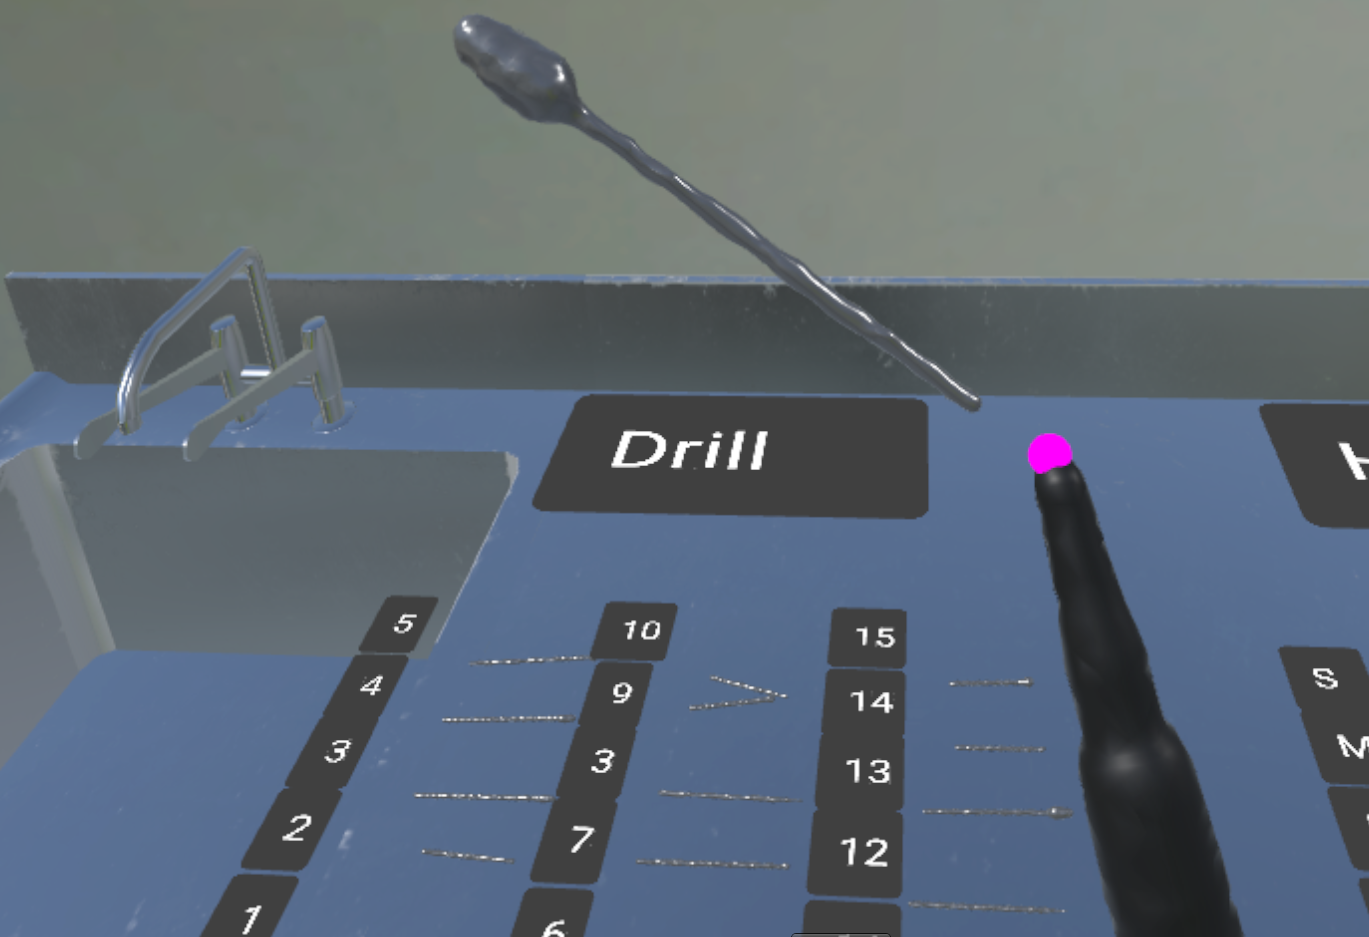
\includegraphics[width=200px]{images/implementation/features/procedures/drilling_attachment.png}
    \caption{\label{fig::FeatureDrillingAttachments}Process of attaching drill bit to the drill handle. With the right hand, the user performs the indicate action by touching 
    the respective button. With the other hand, the bit is picked up by grabbing it and moved into the pink sphere to attach the attachment.}
\end{figure}

In total, there are fifteen bits which can be used as an attachment for the drilling procedure.
Bits are modeled after their real counterparts in UHA.
They differ in size, length and width.
A visual signal is shown to the user while the indicate action is performed on the hand holding the drill handle.
By moving a drill bit to the visual indicator, the bit is attached to the handle (Figure \ref{fig::FeatureDrillingAttachments}).
Swapping out bits is performed by simply moving another bit into the indicator.
To perform the procedure, the drill handle must have a bit attached. 

\begin{figure}[ht]
    \centering
    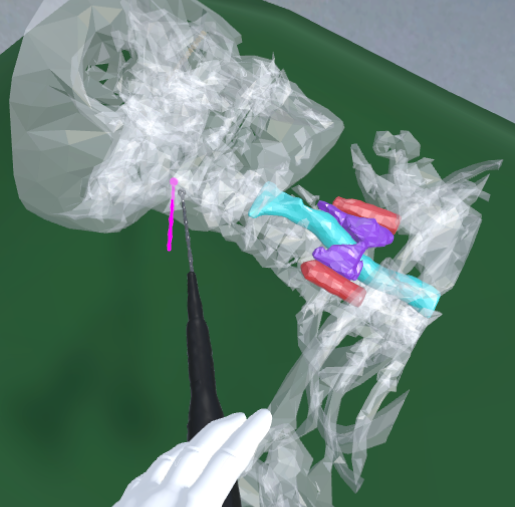
\includegraphics[width=200px]{images/implementation/features/procedures/drilling.png}
    \caption{\label{fig::FeatureDrilling}Drilling procedure. The pink object represents the last performed step, which was performed using the currently selected tool by pressing 
    the respective button all the way.}
\end{figure}

By triggering the perform action of the hand holding the drill, a copy of the currently attached drill bit is created and added to the project case. 
This copy has a different material, i.e. a pink material, to indicate that it is part of the project case (Figure \ref{fig::FeatureDrilling}).
Additionally, textual information about the currently attached drill bit will be stored in the project case, so that the exact procedure can be reproduced later (Requirements \ref{req::N3}, \ref{req::N5}).
The drill bit will not be removed on performing a procedure, so that multiple drilling steps can be performed consecutively.
When the drill is no longer needed, it can either be placed back on the instrument tray or the operating table for quick access.
Note that any instrument, excluding the osteosynthesis plates described later, can be placed anywhere in the OT.
\paragraph{Chiseling}

The \textbf{chiseling} procedure has two parts to it.
First, with one hand a chisel has to be chosen.
Users have a choice between a small, medium, large and extra large chisel to perform the procedure.
With the other hand, users then have to pick up the hammer.
Since this procedure requires users to hold two surgical instruments at the same time, this procedure can get cumbersome.
However, users can easily avoid this by placing the instruments on the operating table in the middle of the OT and repositioning afterwards (Figure \ref{fig::ChiselPrepare}).

\begin{figure}[ht]
    \centering
    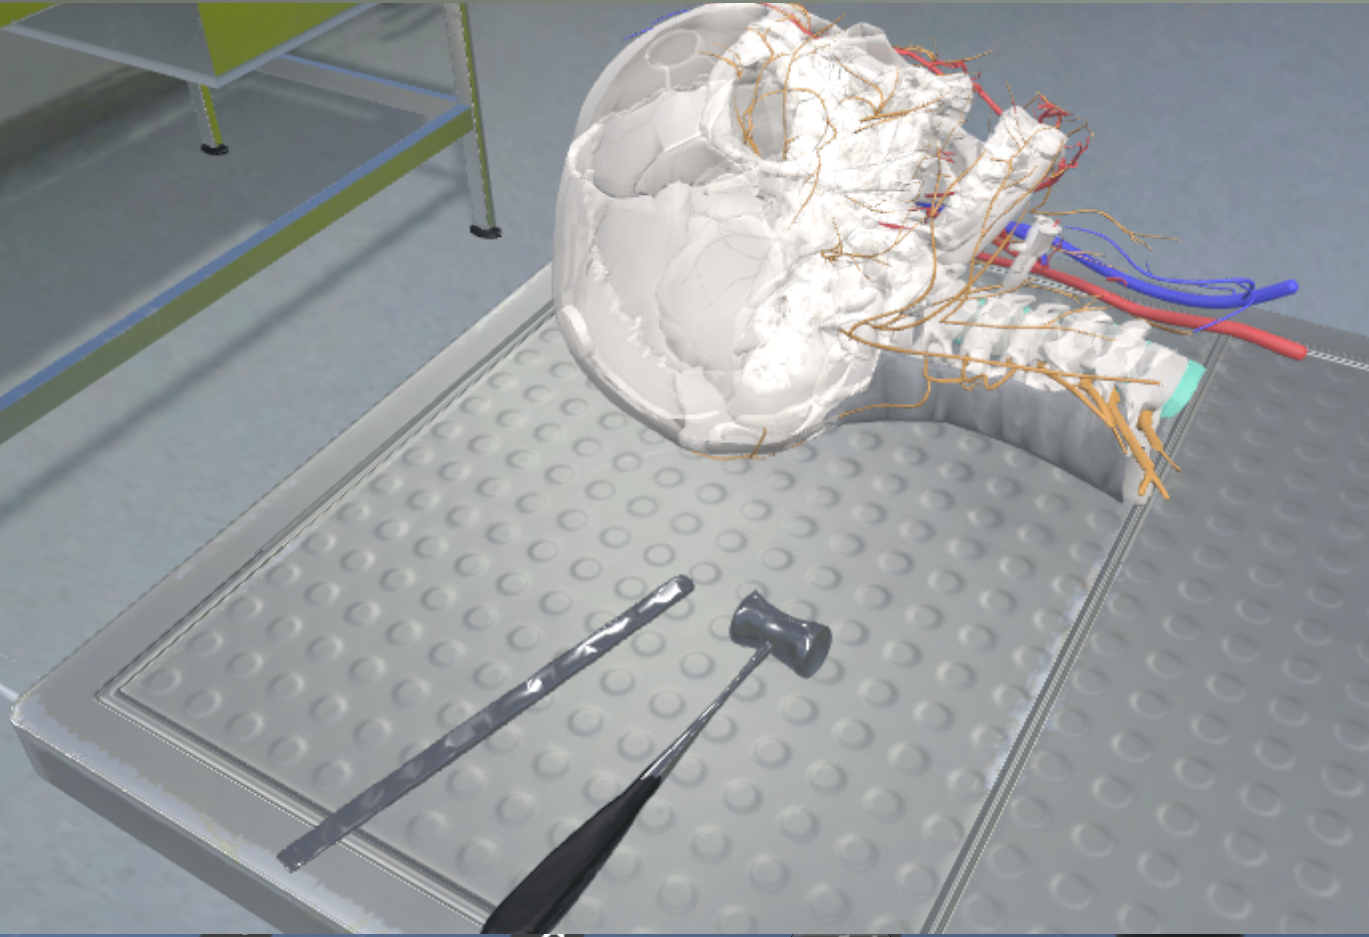
\includegraphics[width=\linewidth]{images/implementation/features/procedures/chisel_prepare.png}
    \caption{\label{fig::ChiselPrepare}The user prepares for the chiseling procedure by placing the instruments on the OT where the patient is located.
    indicators with the hammer in the other hand to perform the procedure.}
\end{figure}

When users have the perfect viewpoint, they can take up both instruments once again and start the procedure.
By pressing the indicate button on the hand where the chisel is located, rectangular indications at the top and bottom end of the chisel are shown to the user.
While these indications are active, the user has to perform a hammering motion with the hand holding the hammer.

\begin{figure}[ht]
    \centering
    \begin{minipage}{.5\textwidth}
      \centering
      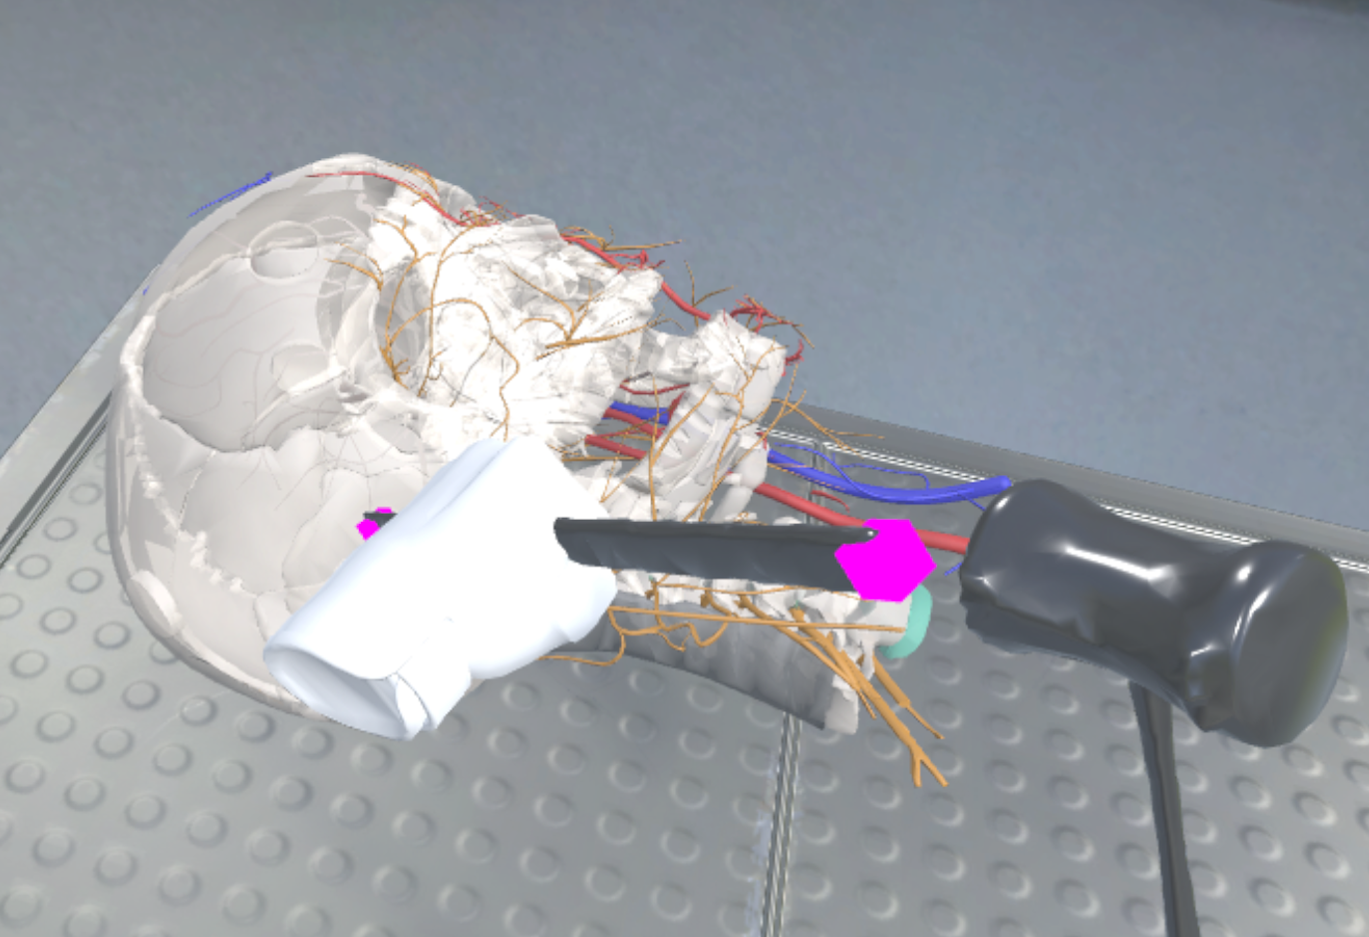
\includegraphics[width=0.99\linewidth]{images/implementation/features/procedures/chisel_1.png}
    \end{minipage}%
    \begin{minipage}{.5\textwidth}
      \centering
      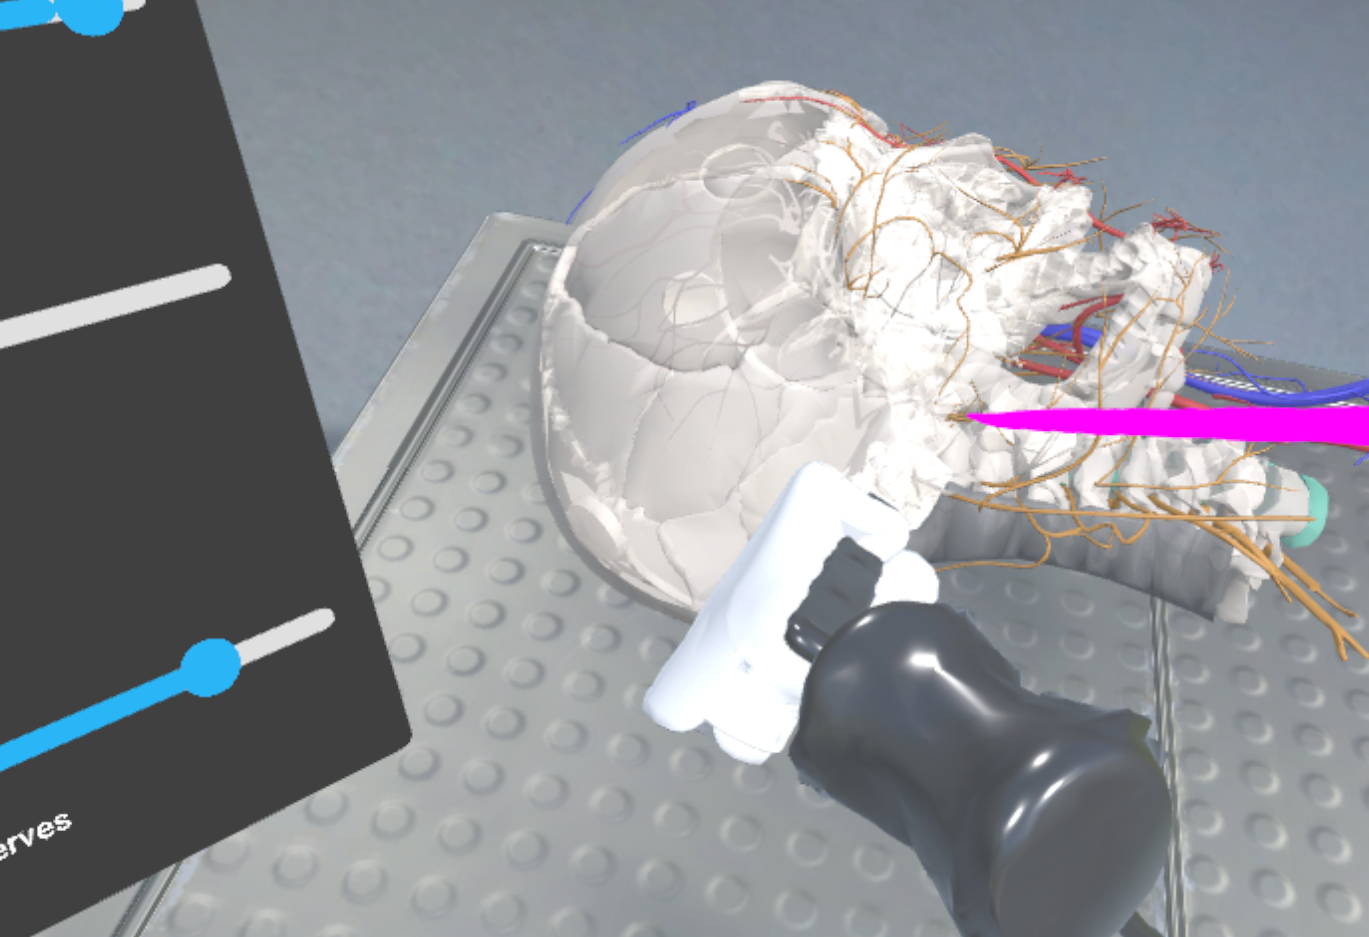
\includegraphics[width=0.99\linewidth]{images/implementation/features/procedures/chisel_2.png}
    \end{minipage}
    \caption{\label{fig::ChiselProcedure}Process of the chiseling procedure. Left: The users uses the indicate action with his left hand in preparation for the procedure. Right: After hammering on the indication on the chisel, the procedure has been performed and a step is generated.}
\end{figure}

When they hit the rectangular indicators located on the chisel, the chiseling procedure step is added to the project case in form of a modified copy of the hold chisel (Figure \ref{fig::ChiselProcedure}).
Here, information about the performed step is also included in the form of chisel size used for the procedure. 
\paragraph{Sawing}

\begin{figure}[ht]
    \centering
    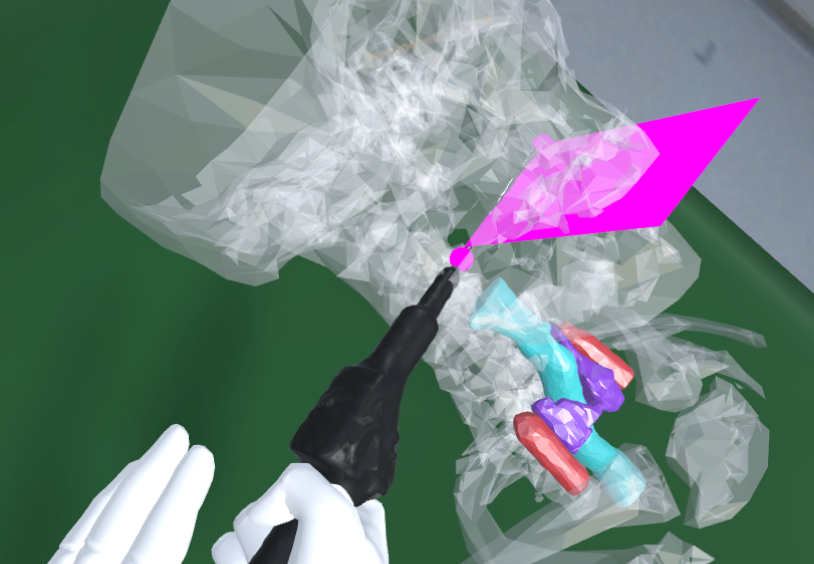
\includegraphics[width=200px]{images/implementation/features/procedures/bonesaw.png}
    \caption{\label{fig::FeatureBoneSaw}Bonesaw Procedure}
\end{figure}

The \textbf{sawing} procedure is performed by picking up the bonesaw.
Touch the controller will show two indications to the user (Figure \ref{fig::FeatureBoneSaw}).
The procedure is performed by first pressing down the trigger button and then letting go of it.
When letting go of the trigger button, a two dimensianal plane is created in the three dimensional space by using four points.
Two of these points are created when pressing down, and the other two when letting go of the trigger button.
A plane is then created with which the user can reproduce the way in which the bonesaw has been moved.
Arbitrary cutting shapes can be created by breaking them down into two-dimensional shapes and performing multiple movements.
\paragraph{Milling}

\begin{figure}[ht]
    \centering
    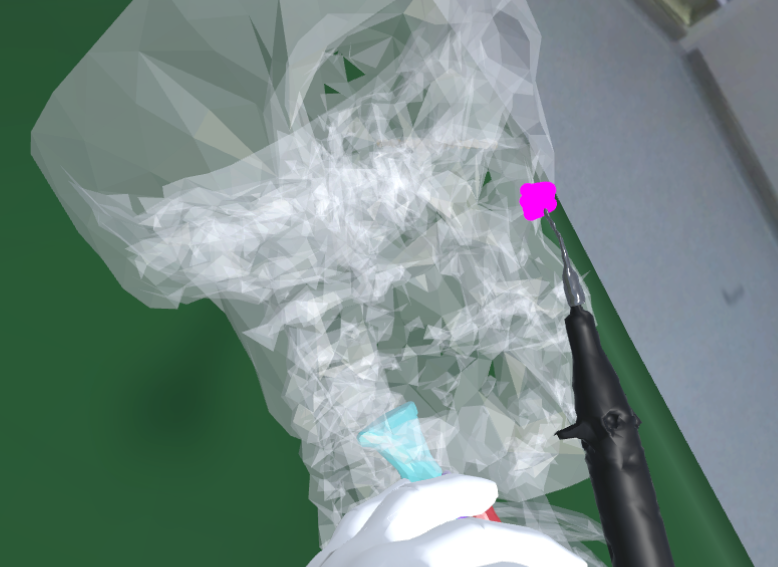
\includegraphics[width=200px]{images/implementation/features/procedures/piezo.png}
    \caption{\label{fig::FeaturePiezo}Milling procedure. Holding down the trigger button will draw little spheres until the button is released. The resulting object represents the volumetric space which is to be milled.}
\end{figure}

The \textbf{milling} operation is performed by grabbing the piezo instrument.
The indicator for the piezo is at the tip of the instrument, indicating which area will be milled.
While the "perform" button is being held down, little spheres are being drawn at the tip of the instrument \ref{fig::FeaturePiezo}.
When the button is released, the shapes are combined into a single 3D model and added as a project step.
The resulting object represents the volumetric space which has to be milled in the procedure.
The procedure can be reconstructed by "milling" the same 3D space in the virtual operating room.
\begin{figure}[ht!]
    \centering
    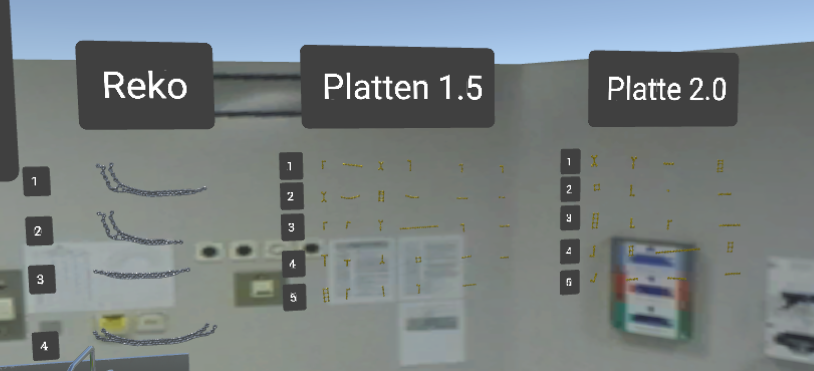
\includegraphics[width=\linewidth]{images/implementation/features/procedures/metal_plates_1.png}
    \caption{\label{fig::FeatureMetalPlate} Osteosynthesis Plates Overview}
\end{figure}

The osteosynthesis plates procedure consists of two steps before adding it as a step to the project case.
First, users have to chose which plate to use (Figure \ref{fig::FeatureMetalPlate}).
The user can chose from four reconstruction plates, 29 1.5mm plates and 20 2.0mm plates (Firma Angeben, osteosynthesis plates).
The optimal plates to use vary due to the pathology of the patient and the previously performed procedures.
After selecting the proper plate, a number of indicators will show to the user (Figure \ref{fig::FeatureMetalPlate2}).
In the context of the osteosynthesis plates, these indicators are "control points", with which the user can bend and twist the plates.
Bending and twisting is performed by chosing a control point via hovering them with the users free hand and grabbing them.
Then, the user has to translate and rotate the control point in the desired manner.
\begin{figure}
  \centering
  \begin{minipage}{.5\textwidth}
    \centering
    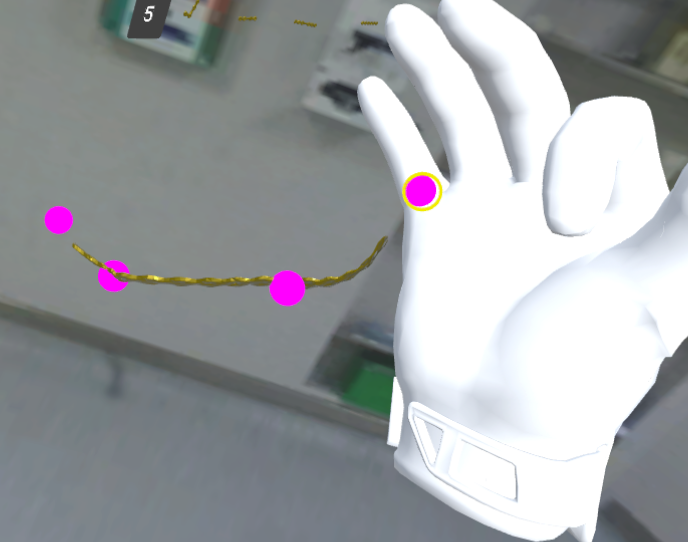
\includegraphics[width=0.95\linewidth]{images/implementation/features/procedures/metal_plates_2.png}
  \end{minipage}%
  \begin{minipage}{.5\textwidth}
    \centering
    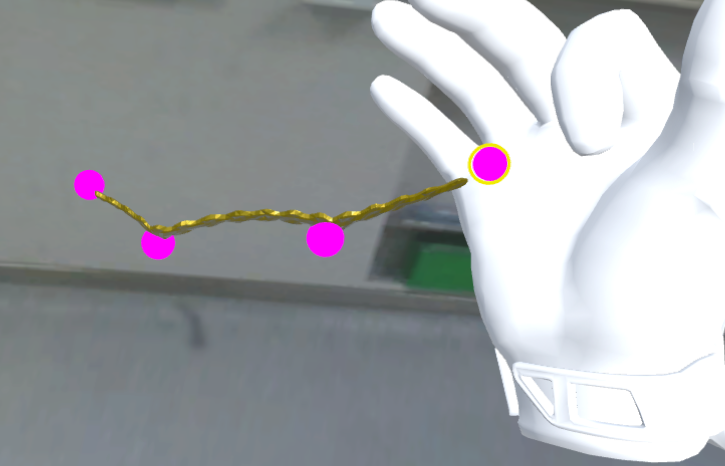
\includegraphics[width=0.95\linewidth]{images/implementation/features/procedures/metal_plates_3.png}
  \end{minipage}
  \caption{\label{fig::FeatureMetalPlate2}Osteosynthesis Plates Modifications. User can translate and rotate "control points" to perform modifications to the plates shape} 
\end{figure}

The user can then observe in which way this has affected the shape of the metal plate and either position the plate on the patient or perform more modifications to the plates via controlpoints.
The correct modification of the metal plates differs quite a lot from real life modifications to the plates.
However even though there is a slight learning curve to it, the modification is consistent and predictable (Figure \ref{fig::FeatureMetalPlate2}).


\begin{figure}[ht!]
    \centering
    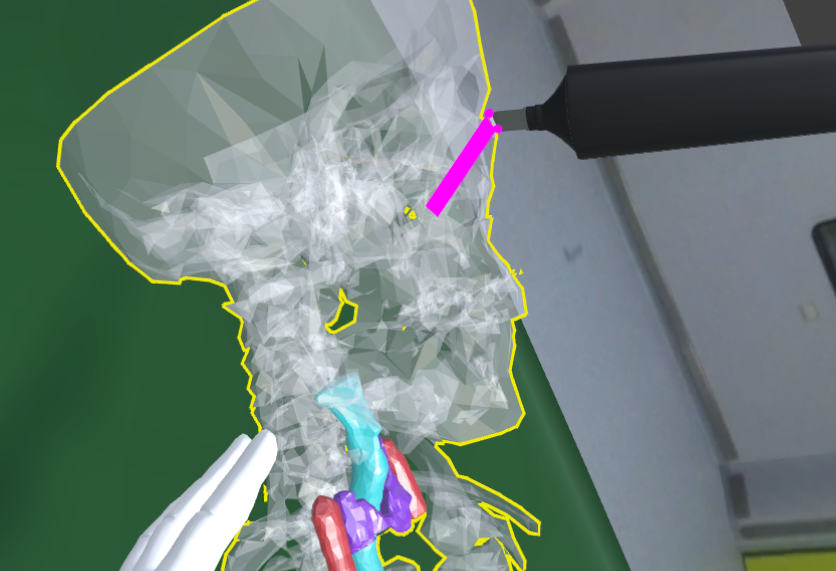
\includegraphics[width=\linewidth]{images/implementation/features/procedures/marker.png}
    \caption{\label{fig::FeatureMarker}Marker Procedure}
\end{figure}

The marking procedure is similar to the bonesaw procedure, meaning that rectangular shapes are drawed into the three dimensianal space (Figure \ref{fig::FeatureMarker}).
However, here the created shapes are much thinner.
In contrast to the bonesaw, the virtual hands of the user are also disabled here.
This way, the user can decide to hold the marker in the optimal way.
Since the main objective is marking specific spots on the patient, this is the natural approach.

\chapter{\label{chap::Implementation}Implementation}
At this point, the aforementioned six procedures are implemented in the system.
However, as described in Section \ref{sec::Architecture}, the system is extensible in the regard that new instruments can be implemented.
Currently, the implemented instruments are based on the workflow of OMF surgeons of the UHA: Users can perform drilling, hammer and chisel, bonesaw and milling operations.
Additionally, users can place markings and osteosynthesis plates on the virtual patient.
\\ To perform procedures, a project case has to be loaded first, as described in Section \ref{sec::GraphicalUserInterface}.
In the sense of SteamVRs interaction system described in Section \ref{sec::Architecture}, for each procedure there is an 'indicate' action when the user touches the 'perform' button, as well as an 'perform' action when the user presses the button all the way.
This way, users get a visual feedback when they are about to perform a procedure, as well as having visual indications of where the procedure will start (i.e. tip of the surgical instrument).
After described each procedure individually, how the procedures come together to create the steps for a procedure will be shortly desctribed.
\\ Each procedure will add a step to the project case.
In the sense of the VR-AR-based workflow described in Section \ref{sec::Workflow}, project cases can then be loaded into both parts of the workflow.
The steps are added to the hierarchy of the patient's 3D model and are identified as a step by name.
Through using this kind of approach, extensibility is guaranteed as each new instrument simply has to add some kind of geometry as a step to the project case (Requirements \ref{req::N8}, \ref{req::F3.7}).
It follows that any kind of procedure can then be imported into the AR workflow, even without touching the application.
\\ When a procedure is performed, users get voice feedback confirming that a step has been added to the project case.
Users can also navigate the project cases steps by using the VUIs commands, so that navigation through the steps of the procedure can be done while holding surgical instruments (Requirements \ref{req::N1}, \ref{req::F3.7}).
\\ For some of the surgical instruments, the user representation of the hand will be shown, for others not.
When a surgical instrument has this feature implemented, it is guaranteed that the instrument will always be grabbed and positioned in the same position on the hand, meaning the handgrip will always be the same.
However, in some cases, f.e. sawing with the bonesaw, this feature would prevent users from switching the handgrip of the surgical instrument. 
Therefore, for some instruments, this feature was removed.
Users will not see their virtual hands on the surgical instrument, but can chose to hold it however they want.
The virtual hands will be hidden while holding the instrument, however the instrument still represents the users hand position.
This way, the handgrip of the instrument can be adapted as users see fit.
The decision, on which was decided if hands should be hidden when grabbing an instrument, was made by a trial and error approach with the help of a physician's opinion on whether this features was useful.
The procedure specific implementation will be thoroughly described in the following.

\paragraph{Drilling}

The \textbf{drilling} operation is performed by first picking up the drill handle from the instrument tray via the grabbing action (Figure \ref{fig::FeatureDrillingAttachments}).
Since drills are typically held in a number of different ways, the handgrip of the drill handle is adjustable.
Therefore, the virtual hand will not be displayed while holding the drill.
The instrument tray is located next to the operating table, where the patient's model will initially be positioned.
The drill handle initially has no attachment; users have to attach a drill bit first.

\begin{figure}[ht]
    \centering
    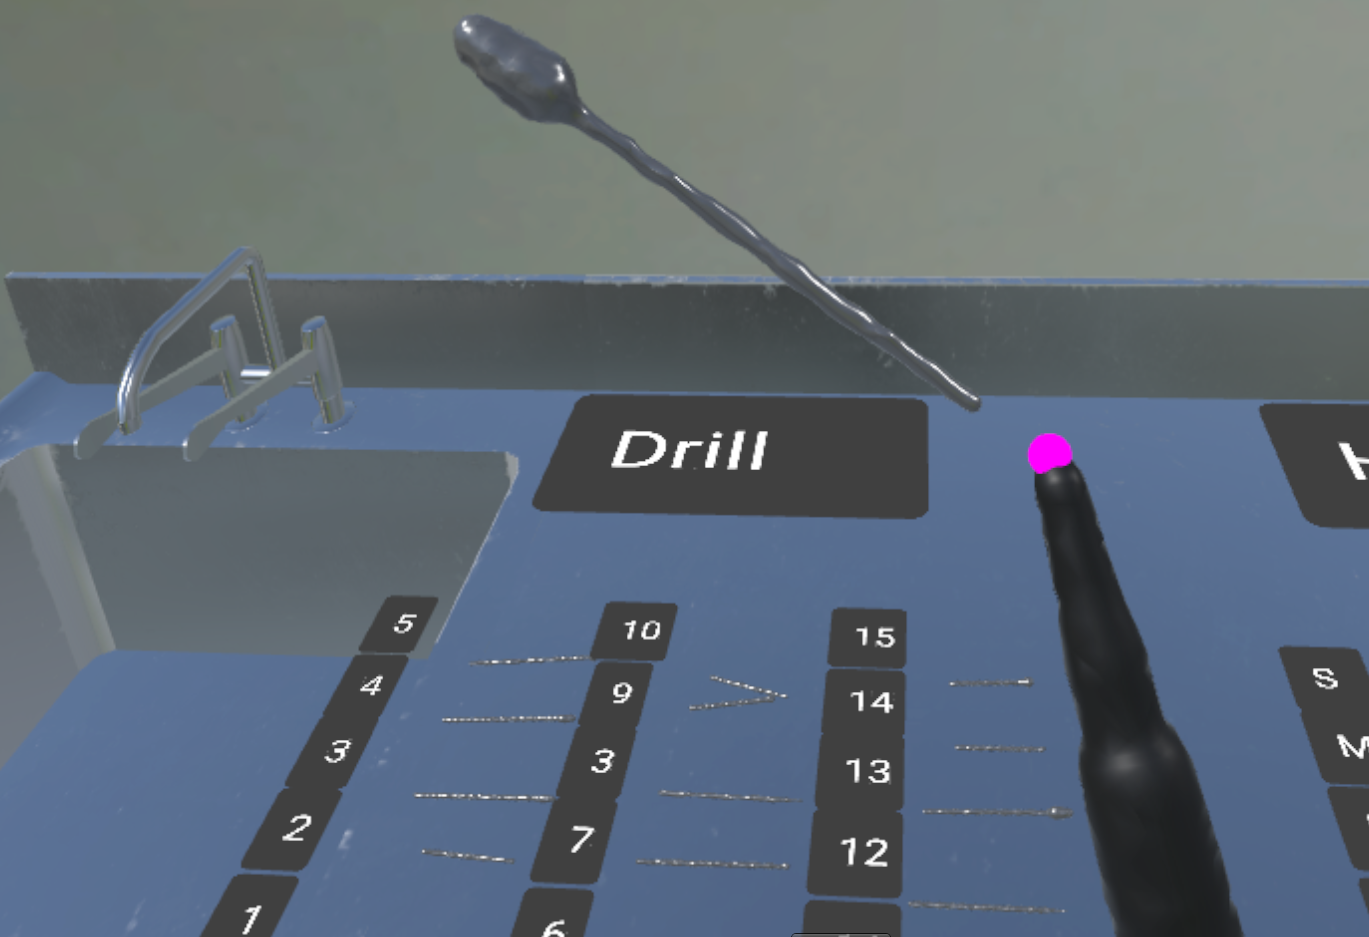
\includegraphics[width=200px]{images/implementation/features/procedures/drilling_attachment.png}
    \caption{\label{fig::FeatureDrillingAttachments}Process of attaching drill bit to the drill handle. With the right hand, the user performs the indicate action by touching 
    the respective button. With the other hand, the bit is picked up by grabbing it and moved into the pink sphere to attach the attachment.}
\end{figure}

In total, there are fifteen bits which can be used as an attachment for the drilling procedure.
Bits are modeled after their real counterparts in UHA.
They differ in size, length and width.
A visual signal is shown to the user while the indicate action is performed on the hand holding the drill handle.
By moving a drill bit to the visual indicator, the bit is attached to the handle (Figure \ref{fig::FeatureDrillingAttachments}).
Swapping out bits is performed by simply moving another bit into the indicator.
To perform the procedure, the drill handle must have a bit attached. 

\begin{figure}[ht]
    \centering
    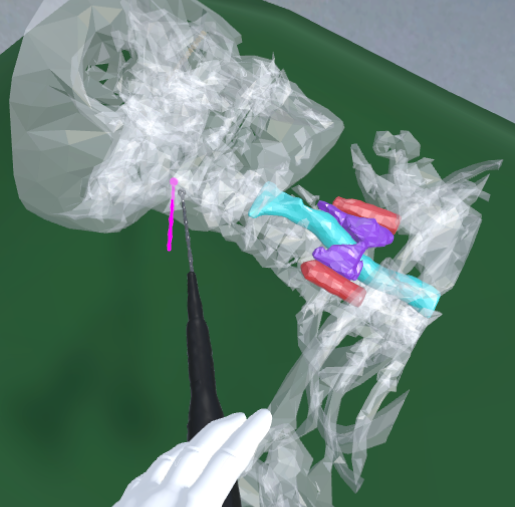
\includegraphics[width=200px]{images/implementation/features/procedures/drilling.png}
    \caption{\label{fig::FeatureDrilling}Drilling procedure. The pink object represents the last performed step, which was performed using the currently selected tool by pressing 
    the respective button all the way.}
\end{figure}

By triggering the perform action of the hand holding the drill, a copy of the currently attached drill bit is created and added to the project case. 
This copy has a different material, i.e. a pink material, to indicate that it is part of the project case (Figure \ref{fig::FeatureDrilling}).
Additionally, textual information about the currently attached drill bit will be stored in the project case, so that the exact procedure can be reproduced later (Requirements \ref{req::N3}, \ref{req::N5}).
The drill bit will not be removed on performing a procedure, so that multiple drilling steps can be performed consecutively.
When the drill is no longer needed, it can either be placed back on the instrument tray or the operating table for quick access.
Note that any instrument, excluding the osteosynthesis plates described later, can be placed anywhere in the OT.
\paragraph{Chiseling}

The \textbf{chiseling} procedure has two parts to it.
First, with one hand a chisel has to be chosen.
Users have a choice between a small, medium, large and extra large chisel to perform the procedure.
With the other hand, users then have to pick up the hammer.
Since this procedure requires users to hold two surgical instruments at the same time, this procedure can get cumbersome.
However, users can easily avoid this by placing the instruments on the operating table in the middle of the OT and repositioning afterwards (Figure \ref{fig::ChiselPrepare}).

\begin{figure}[ht]
    \centering
    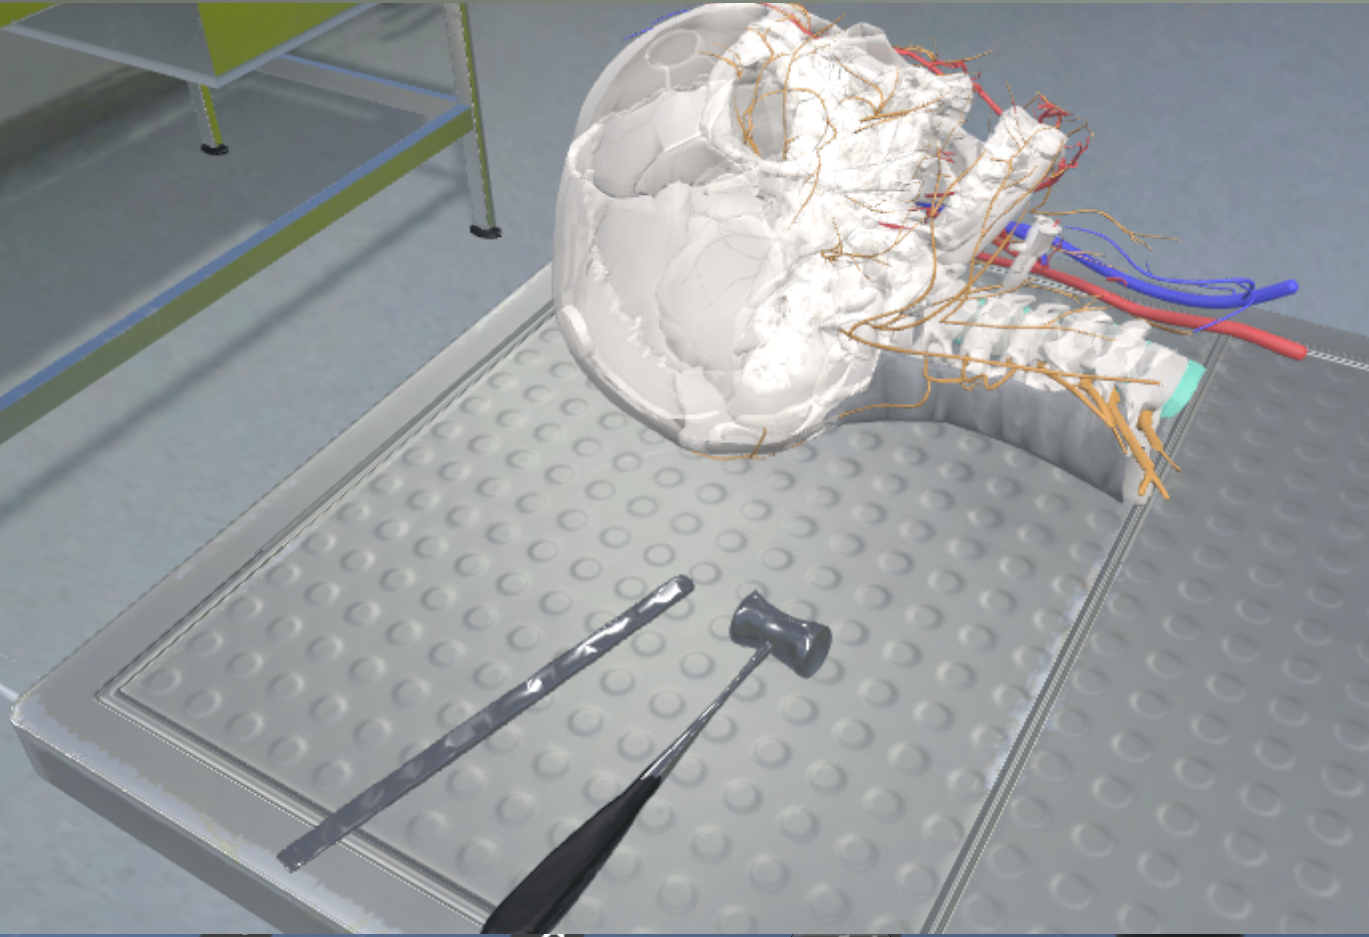
\includegraphics[width=\linewidth]{images/implementation/features/procedures/chisel_prepare.png}
    \caption{\label{fig::ChiselPrepare}The user prepares for the chiseling procedure by placing the instruments on the OT where the patient is located.
    indicators with the hammer in the other hand to perform the procedure.}
\end{figure}

When users have the perfect viewpoint, they can take up both instruments once again and start the procedure.
By pressing the indicate button on the hand where the chisel is located, rectangular indications at the top and bottom end of the chisel are shown to the user.
While these indications are active, the user has to perform a hammering motion with the hand holding the hammer.

\begin{figure}[ht]
    \centering
    \begin{minipage}{.5\textwidth}
      \centering
      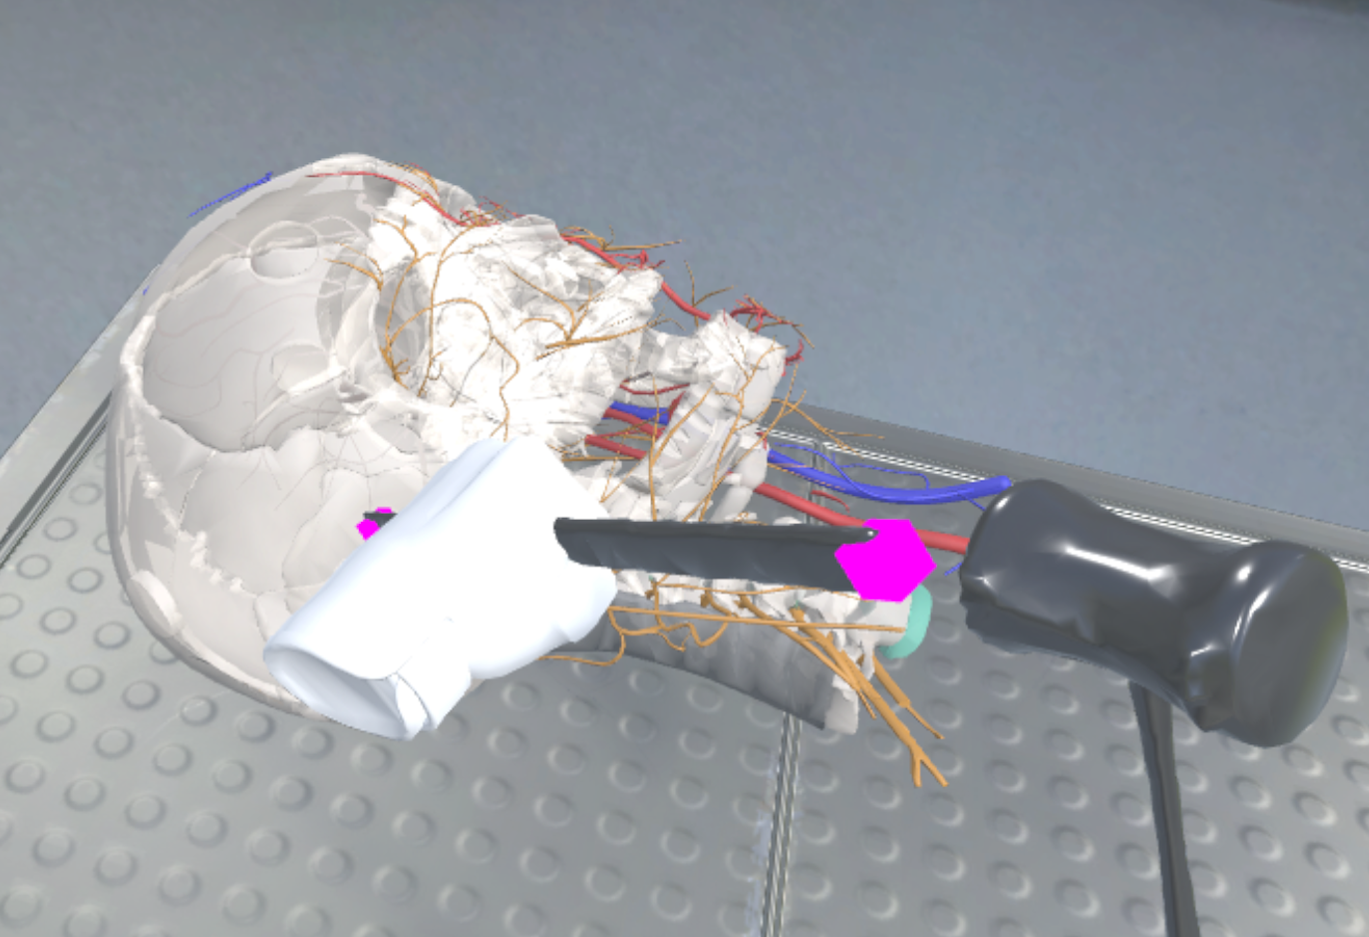
\includegraphics[width=0.99\linewidth]{images/implementation/features/procedures/chisel_1.png}
    \end{minipage}%
    \begin{minipage}{.5\textwidth}
      \centering
      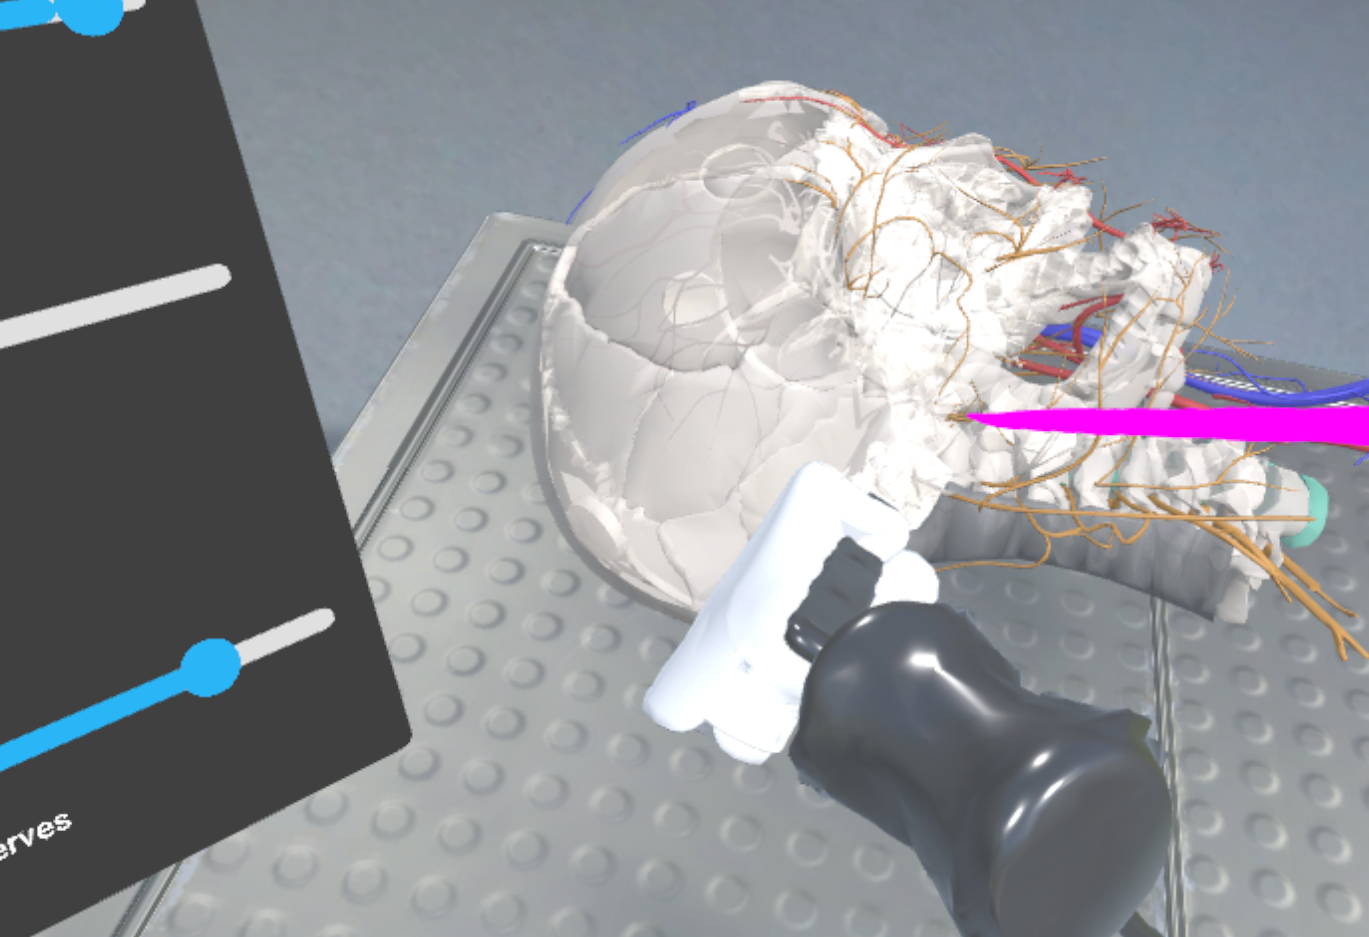
\includegraphics[width=0.99\linewidth]{images/implementation/features/procedures/chisel_2.png}
    \end{minipage}
    \caption{\label{fig::ChiselProcedure}Process of the chiseling procedure. Left: The users uses the indicate action with his left hand in preparation for the procedure. Right: After hammering on the indication on the chisel, the procedure has been performed and a step is generated.}
\end{figure}

When they hit the rectangular indicators located on the chisel, the chiseling procedure step is added to the project case in form of a modified copy of the hold chisel (Figure \ref{fig::ChiselProcedure}).
Here, information about the performed step is also included in the form of chisel size used for the procedure. 
\paragraph{Sawing}

\begin{figure}[ht]
    \centering
    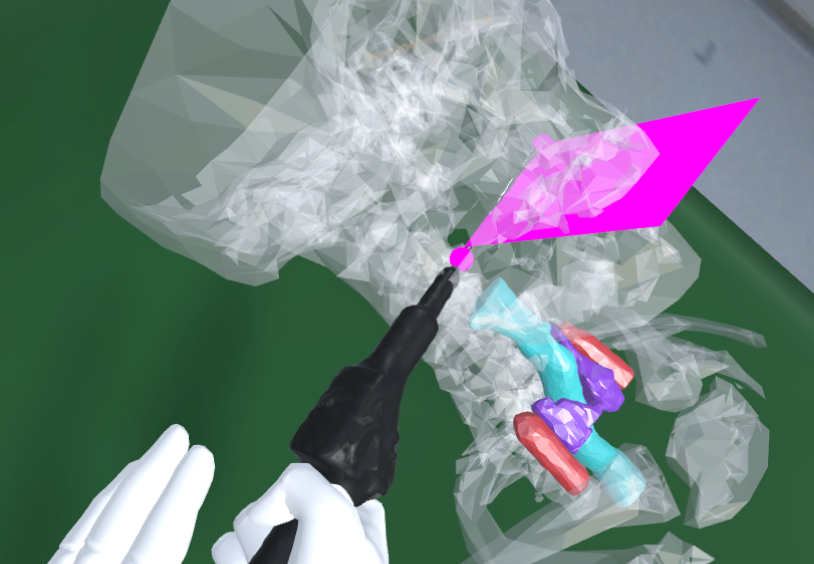
\includegraphics[width=200px]{images/implementation/features/procedures/bonesaw.png}
    \caption{\label{fig::FeatureBoneSaw}Bonesaw Procedure}
\end{figure}

The \textbf{sawing} procedure is performed by picking up the bonesaw.
Touch the controller will show two indications to the user (Figure \ref{fig::FeatureBoneSaw}).
The procedure is performed by first pressing down the trigger button and then letting go of it.
When letting go of the trigger button, a two dimensianal plane is created in the three dimensional space by using four points.
Two of these points are created when pressing down, and the other two when letting go of the trigger button.
A plane is then created with which the user can reproduce the way in which the bonesaw has been moved.
Arbitrary cutting shapes can be created by breaking them down into two-dimensional shapes and performing multiple movements.
\paragraph{Milling}

\begin{figure}[ht]
    \centering
    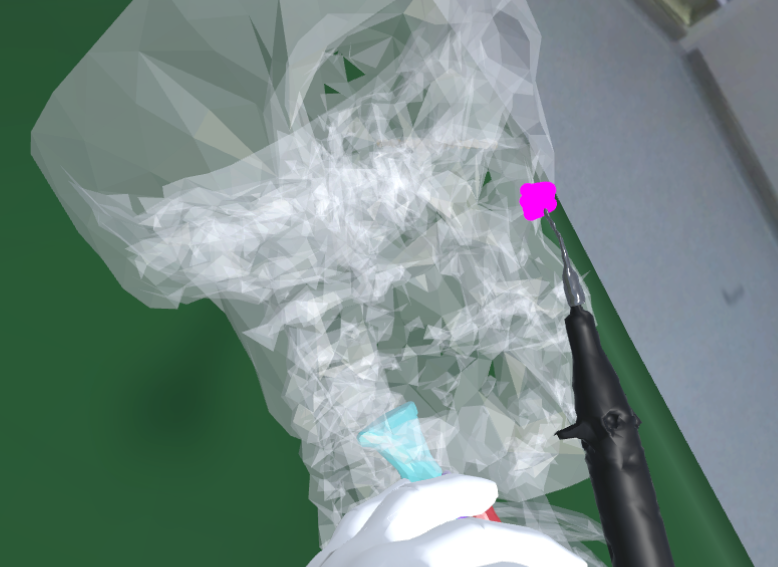
\includegraphics[width=200px]{images/implementation/features/procedures/piezo.png}
    \caption{\label{fig::FeaturePiezo}Milling procedure. Holding down the trigger button will draw little spheres until the button is released. The resulting object represents the volumetric space which is to be milled.}
\end{figure}

The \textbf{milling} operation is performed by grabbing the piezo instrument.
The indicator for the piezo is at the tip of the instrument, indicating which area will be milled.
While the "perform" button is being held down, little spheres are being drawn at the tip of the instrument \ref{fig::FeaturePiezo}.
When the button is released, the shapes are combined into a single 3D model and added as a project step.
The resulting object represents the volumetric space which has to be milled in the procedure.
The procedure can be reconstructed by "milling" the same 3D space in the virtual operating room.
\begin{figure}[ht!]
    \centering
    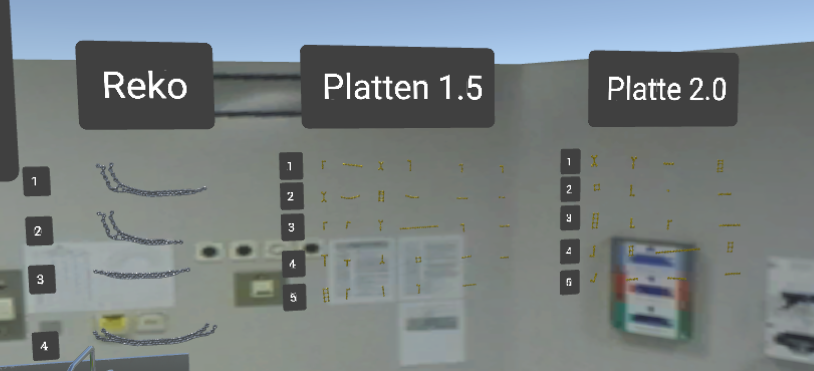
\includegraphics[width=\linewidth]{images/implementation/features/procedures/metal_plates_1.png}
    \caption{\label{fig::FeatureMetalPlate} Osteosynthesis Plates Overview}
\end{figure}

The osteosynthesis plates procedure consists of two steps before adding it as a step to the project case.
First, users have to chose which plate to use (Figure \ref{fig::FeatureMetalPlate}).
The user can chose from four reconstruction plates, 29 1.5mm plates and 20 2.0mm plates (Firma Angeben, osteosynthesis plates).
The optimal plates to use vary due to the pathology of the patient and the previously performed procedures.
After selecting the proper plate, a number of indicators will show to the user (Figure \ref{fig::FeatureMetalPlate2}).
In the context of the osteosynthesis plates, these indicators are "control points", with which the user can bend and twist the plates.
Bending and twisting is performed by chosing a control point via hovering them with the users free hand and grabbing them.
Then, the user has to translate and rotate the control point in the desired manner.
\begin{figure}
  \centering
  \begin{minipage}{.5\textwidth}
    \centering
    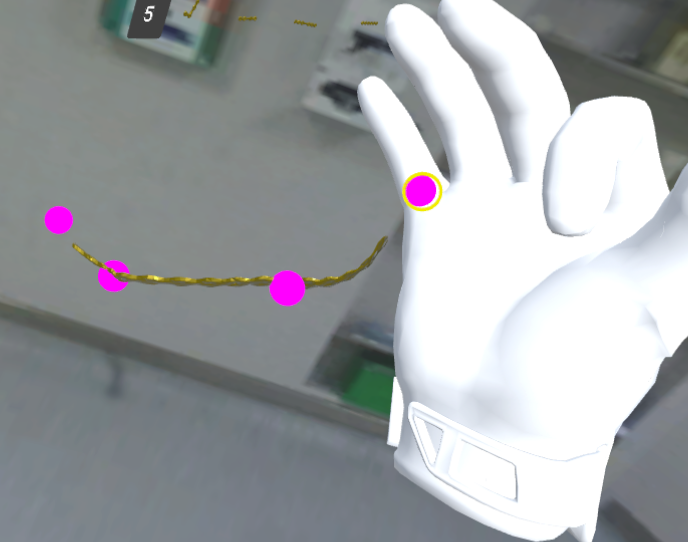
\includegraphics[width=0.95\linewidth]{images/implementation/features/procedures/metal_plates_2.png}
  \end{minipage}%
  \begin{minipage}{.5\textwidth}
    \centering
    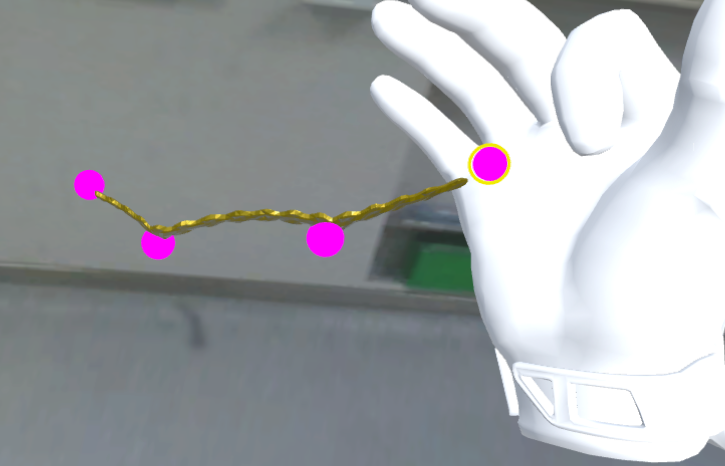
\includegraphics[width=0.95\linewidth]{images/implementation/features/procedures/metal_plates_3.png}
  \end{minipage}
  \caption{\label{fig::FeatureMetalPlate2}Osteosynthesis Plates Modifications. User can translate and rotate "control points" to perform modifications to the plates shape} 
\end{figure}

The user can then observe in which way this has affected the shape of the metal plate and either position the plate on the patient or perform more modifications to the plates via controlpoints.
The correct modification of the metal plates differs quite a lot from real life modifications to the plates.
However even though there is a slight learning curve to it, the modification is consistent and predictable (Figure \ref{fig::FeatureMetalPlate2}).


\begin{figure}[ht!]
    \centering
    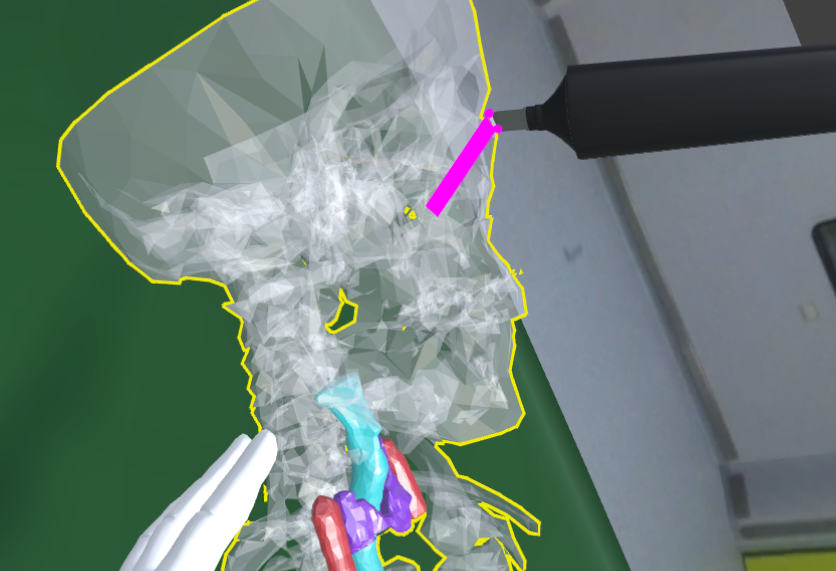
\includegraphics[width=\linewidth]{images/implementation/features/procedures/marker.png}
    \caption{\label{fig::FeatureMarker}Marker Procedure}
\end{figure}

The marking procedure is similar to the bonesaw procedure, meaning that rectangular shapes are drawed into the three dimensianal space (Figure \ref{fig::FeatureMarker}).
However, here the created shapes are much thinner.
In contrast to the bonesaw, the virtual hands of the user are also disabled here.
This way, the user can decide to hold the marker in the optimal way.
Since the main objective is marking specific spots on the patient, this is the natural approach.

\chapter{\label{chap::Evaluation}Evaluation}
At this point, the aforementioned six procedures are implemented in the system.
However, as described in Section \ref{sec::Architecture}, the system is extensible in the regard that new instruments can be implemented.
Currently, the implemented instruments are based on the workflow of OMF surgeons of the UHA: Users can perform drilling, hammer and chisel, bonesaw and milling operations.
Additionally, users can place markings and osteosynthesis plates on the virtual patient.
\\ To perform procedures, a project case has to be loaded first, as described in Section \ref{sec::GraphicalUserInterface}.
In the sense of SteamVRs interaction system described in Section \ref{sec::Architecture}, for each procedure there is an 'indicate' action when the user touches the 'perform' button, as well as an 'perform' action when the user presses the button all the way.
This way, users get a visual feedback when they are about to perform a procedure, as well as having visual indications of where the procedure will start (i.e. tip of the surgical instrument).
After described each procedure individually, how the procedures come together to create the steps for a procedure will be shortly desctribed.
\\ Each procedure will add a step to the project case.
In the sense of the VR-AR-based workflow described in Section \ref{sec::Workflow}, project cases can then be loaded into both parts of the workflow.
The steps are added to the hierarchy of the patient's 3D model and are identified as a step by name.
Through using this kind of approach, extensibility is guaranteed as each new instrument simply has to add some kind of geometry as a step to the project case (Requirements \ref{req::N8}, \ref{req::F3.7}).
It follows that any kind of procedure can then be imported into the AR workflow, even without touching the application.
\\ When a procedure is performed, users get voice feedback confirming that a step has been added to the project case.
Users can also navigate the project cases steps by using the VUIs commands, so that navigation through the steps of the procedure can be done while holding surgical instruments (Requirements \ref{req::N1}, \ref{req::F3.7}).
\\ For some of the surgical instruments, the user representation of the hand will be shown, for others not.
When a surgical instrument has this feature implemented, it is guaranteed that the instrument will always be grabbed and positioned in the same position on the hand, meaning the handgrip will always be the same.
However, in some cases, f.e. sawing with the bonesaw, this feature would prevent users from switching the handgrip of the surgical instrument. 
Therefore, for some instruments, this feature was removed.
Users will not see their virtual hands on the surgical instrument, but can chose to hold it however they want.
The virtual hands will be hidden while holding the instrument, however the instrument still represents the users hand position.
This way, the handgrip of the instrument can be adapted as users see fit.
The decision, on which was decided if hands should be hidden when grabbing an instrument, was made by a trial and error approach with the help of a physician's opinion on whether this features was useful.
The procedure specific implementation will be thoroughly described in the following.

\paragraph{Drilling}

The \textbf{drilling} operation is performed by first picking up the drill handle from the instrument tray via the grabbing action (Figure \ref{fig::FeatureDrillingAttachments}).
Since drills are typically held in a number of different ways, the handgrip of the drill handle is adjustable.
Therefore, the virtual hand will not be displayed while holding the drill.
The instrument tray is located next to the operating table, where the patient's model will initially be positioned.
The drill handle initially has no attachment; users have to attach a drill bit first.

\begin{figure}[ht]
    \centering
    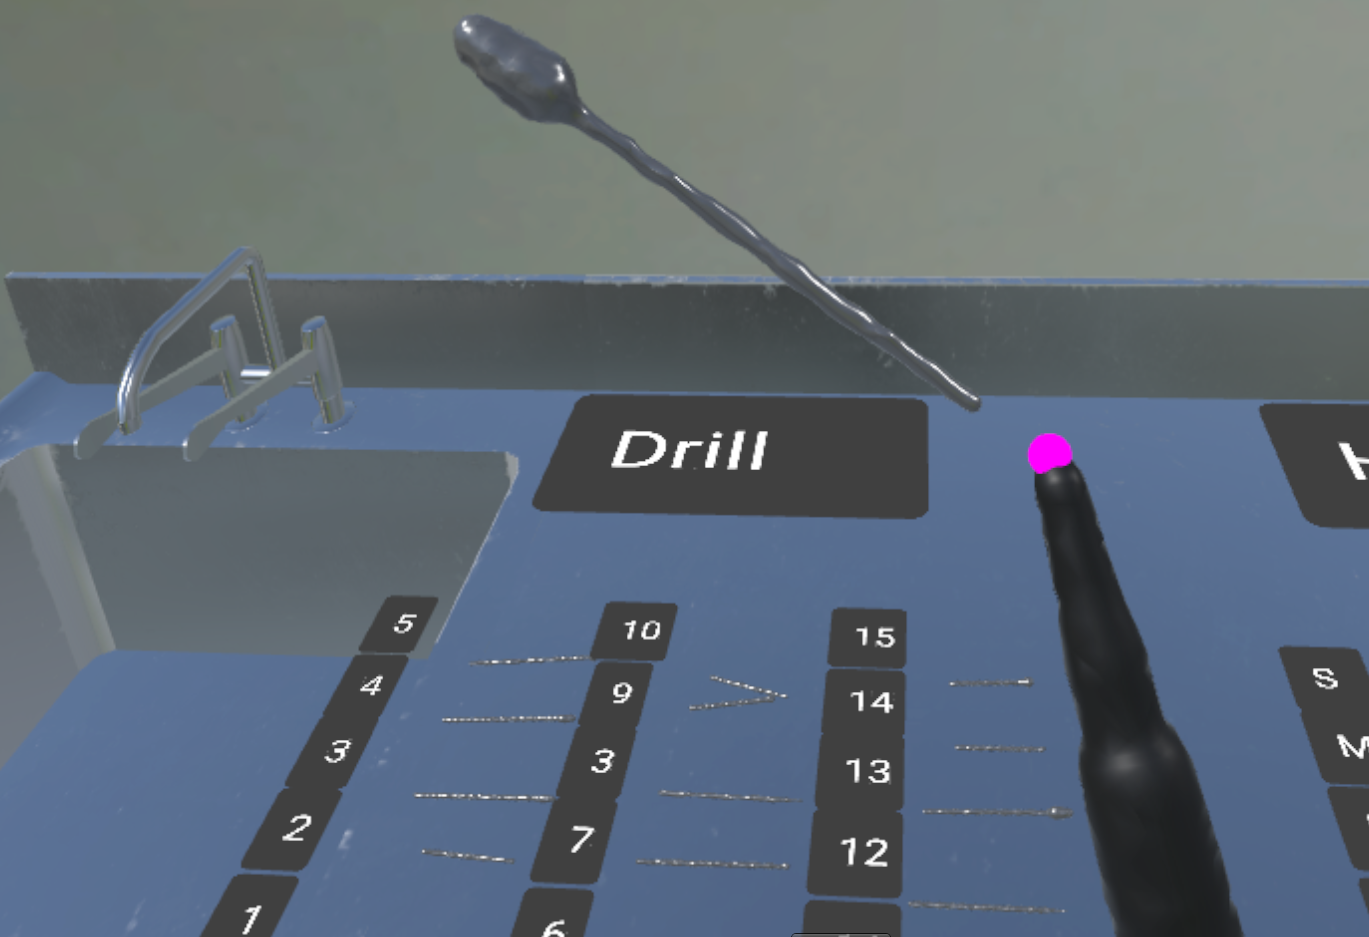
\includegraphics[width=200px]{images/implementation/features/procedures/drilling_attachment.png}
    \caption{\label{fig::FeatureDrillingAttachments}Process of attaching drill bit to the drill handle. With the right hand, the user performs the indicate action by touching 
    the respective button. With the other hand, the bit is picked up by grabbing it and moved into the pink sphere to attach the attachment.}
\end{figure}

In total, there are fifteen bits which can be used as an attachment for the drilling procedure.
Bits are modeled after their real counterparts in UHA.
They differ in size, length and width.
A visual signal is shown to the user while the indicate action is performed on the hand holding the drill handle.
By moving a drill bit to the visual indicator, the bit is attached to the handle (Figure \ref{fig::FeatureDrillingAttachments}).
Swapping out bits is performed by simply moving another bit into the indicator.
To perform the procedure, the drill handle must have a bit attached. 

\begin{figure}[ht]
    \centering
    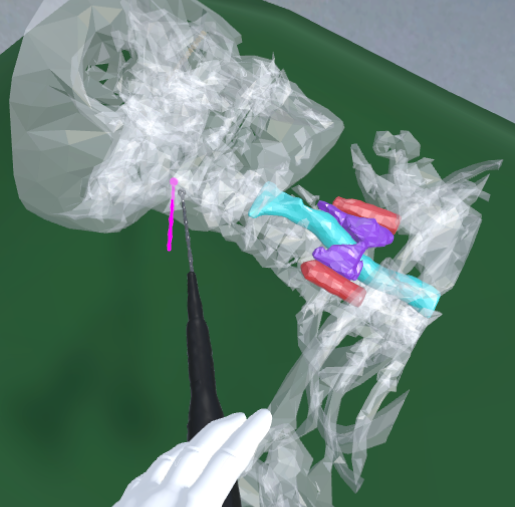
\includegraphics[width=200px]{images/implementation/features/procedures/drilling.png}
    \caption{\label{fig::FeatureDrilling}Drilling procedure. The pink object represents the last performed step, which was performed using the currently selected tool by pressing 
    the respective button all the way.}
\end{figure}

By triggering the perform action of the hand holding the drill, a copy of the currently attached drill bit is created and added to the project case. 
This copy has a different material, i.e. a pink material, to indicate that it is part of the project case (Figure \ref{fig::FeatureDrilling}).
Additionally, textual information about the currently attached drill bit will be stored in the project case, so that the exact procedure can be reproduced later (Requirements \ref{req::N3}, \ref{req::N5}).
The drill bit will not be removed on performing a procedure, so that multiple drilling steps can be performed consecutively.
When the drill is no longer needed, it can either be placed back on the instrument tray or the operating table for quick access.
Note that any instrument, excluding the osteosynthesis plates described later, can be placed anywhere in the OT.
\paragraph{Chiseling}

The \textbf{chiseling} procedure has two parts to it.
First, with one hand a chisel has to be chosen.
Users have a choice between a small, medium, large and extra large chisel to perform the procedure.
With the other hand, users then have to pick up the hammer.
Since this procedure requires users to hold two surgical instruments at the same time, this procedure can get cumbersome.
However, users can easily avoid this by placing the instruments on the operating table in the middle of the OT and repositioning afterwards (Figure \ref{fig::ChiselPrepare}).

\begin{figure}[ht]
    \centering
    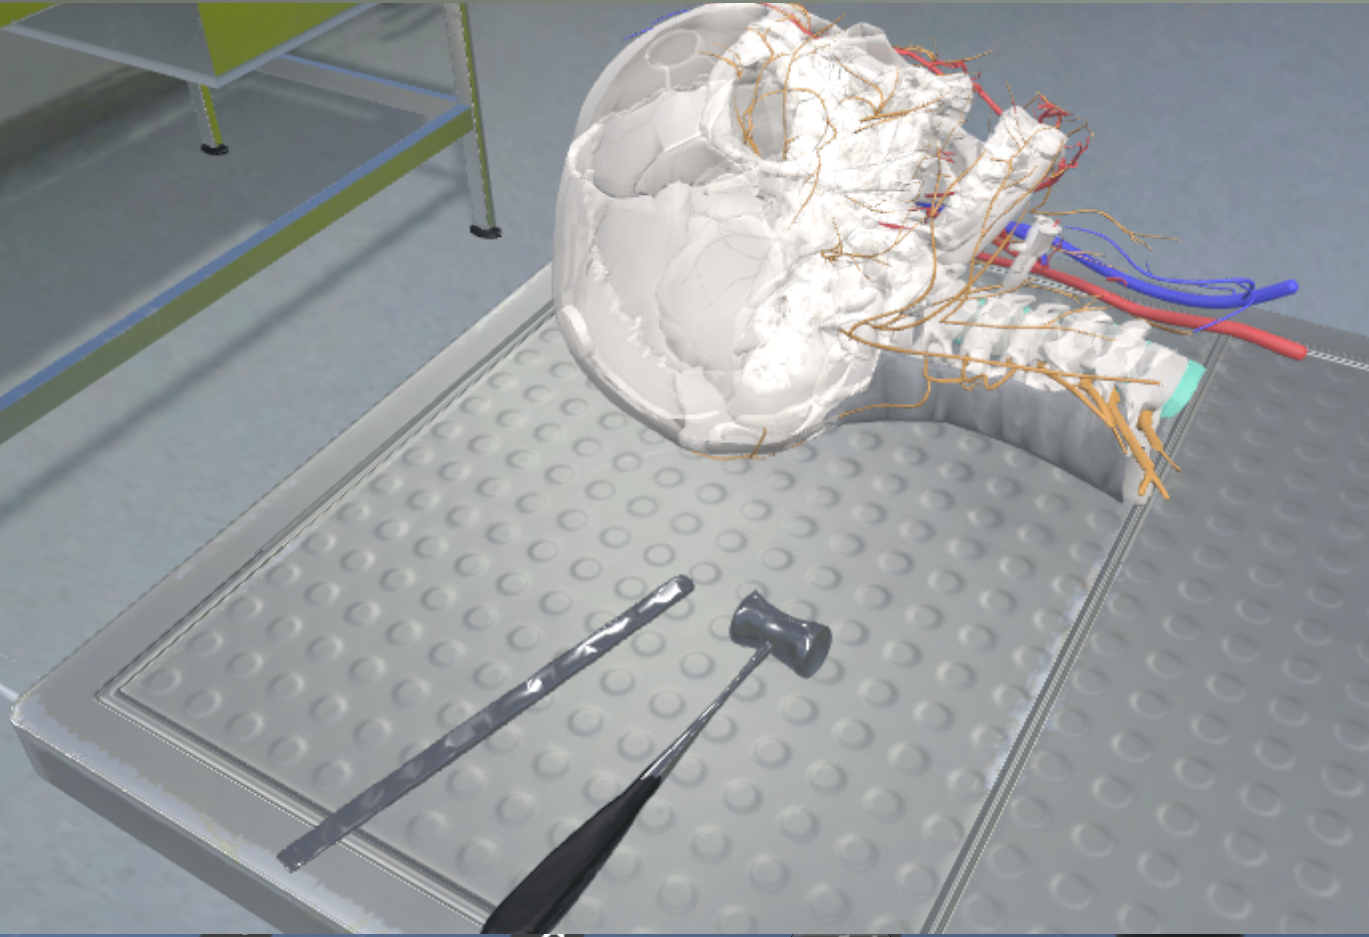
\includegraphics[width=\linewidth]{images/implementation/features/procedures/chisel_prepare.png}
    \caption{\label{fig::ChiselPrepare}The user prepares for the chiseling procedure by placing the instruments on the OT where the patient is located.
    indicators with the hammer in the other hand to perform the procedure.}
\end{figure}

When users have the perfect viewpoint, they can take up both instruments once again and start the procedure.
By pressing the indicate button on the hand where the chisel is located, rectangular indications at the top and bottom end of the chisel are shown to the user.
While these indications are active, the user has to perform a hammering motion with the hand holding the hammer.

\begin{figure}[ht]
    \centering
    \begin{minipage}{.5\textwidth}
      \centering
      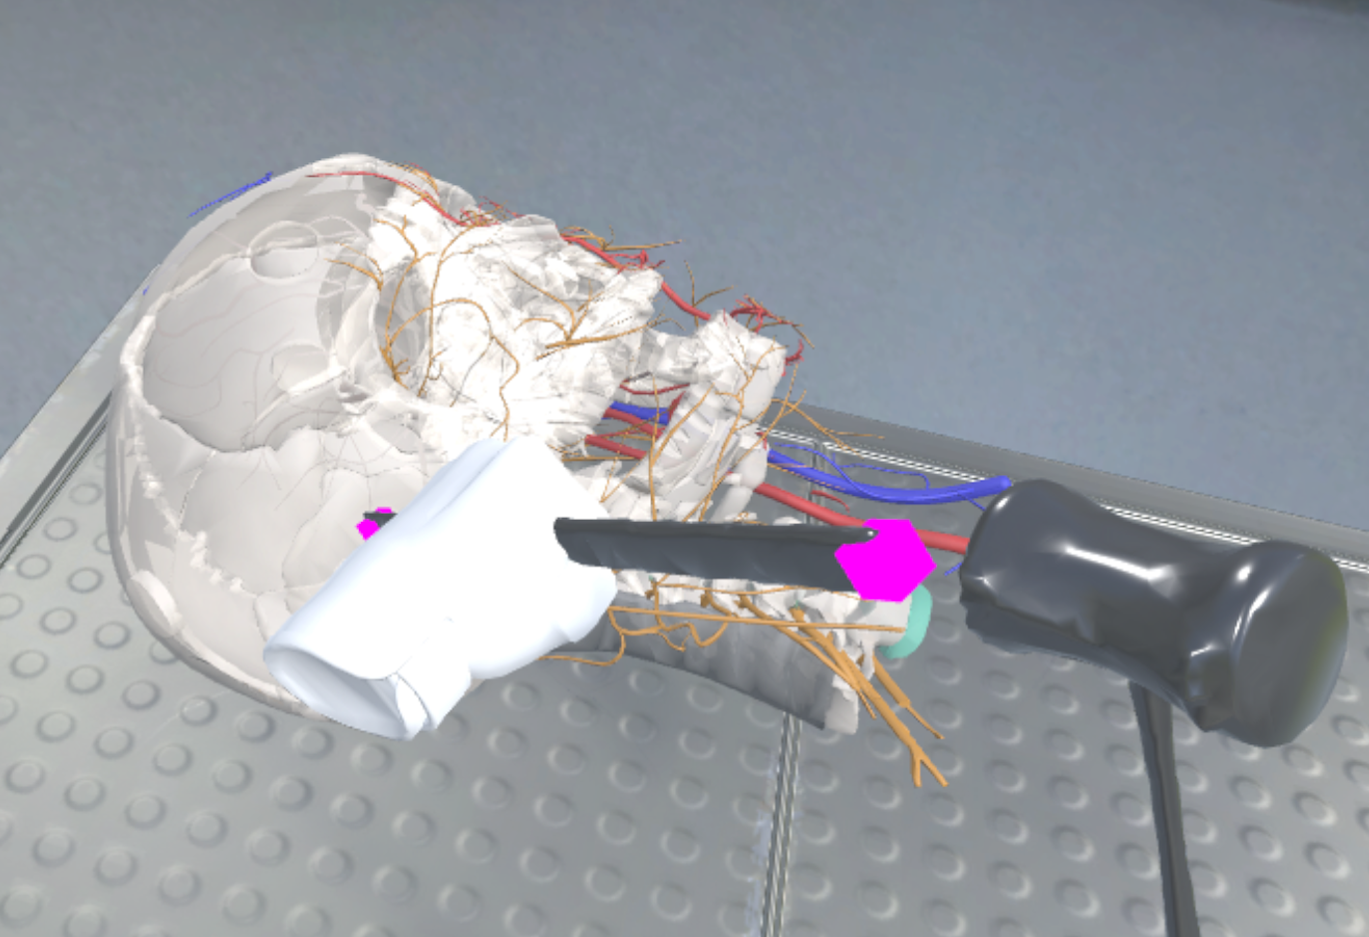
\includegraphics[width=0.99\linewidth]{images/implementation/features/procedures/chisel_1.png}
    \end{minipage}%
    \begin{minipage}{.5\textwidth}
      \centering
      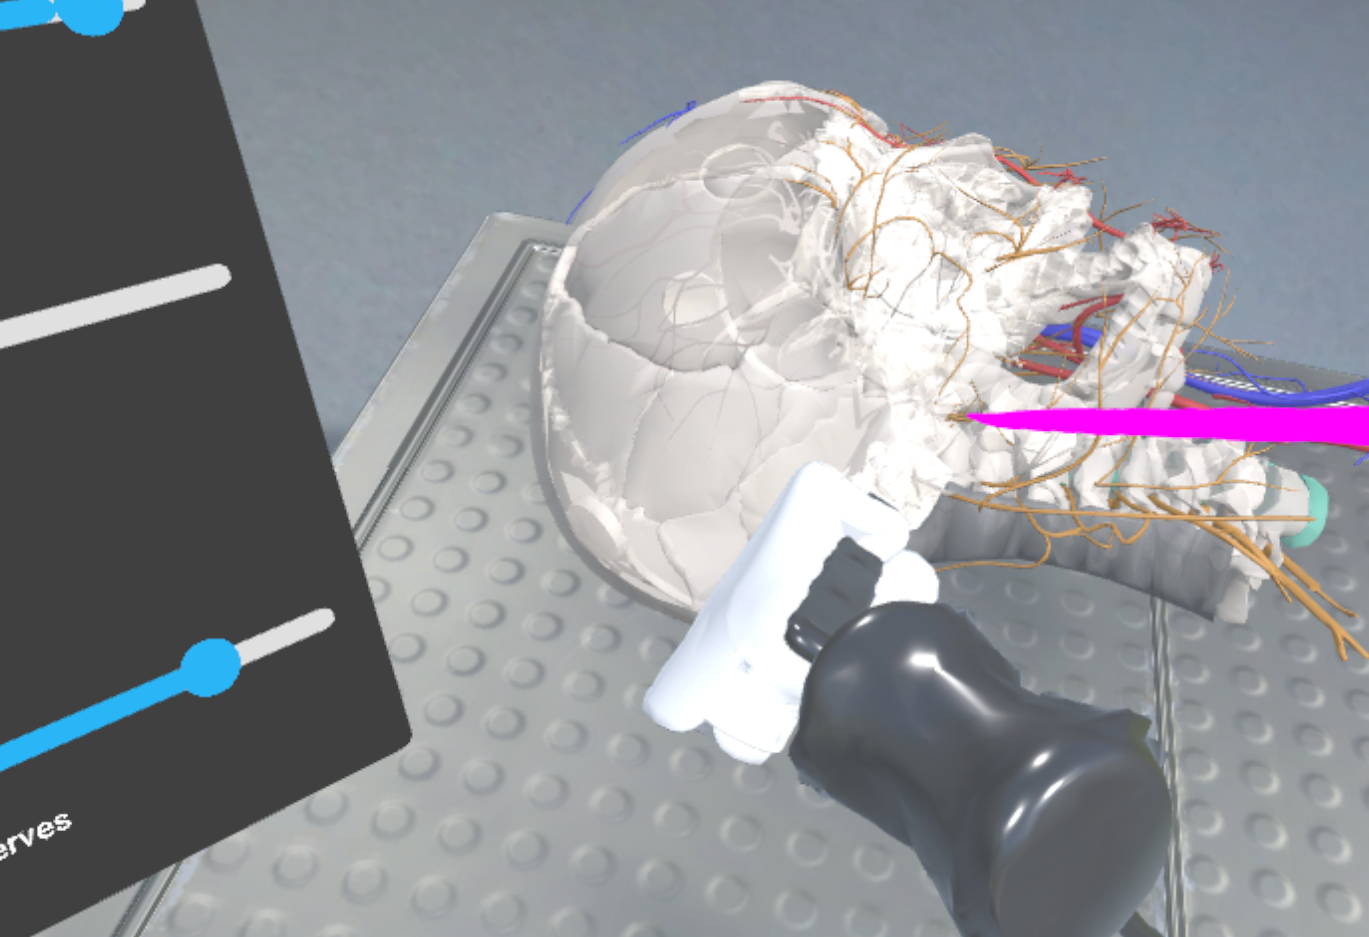
\includegraphics[width=0.99\linewidth]{images/implementation/features/procedures/chisel_2.png}
    \end{minipage}
    \caption{\label{fig::ChiselProcedure}Process of the chiseling procedure. Left: The users uses the indicate action with his left hand in preparation for the procedure. Right: After hammering on the indication on the chisel, the procedure has been performed and a step is generated.}
\end{figure}

When they hit the rectangular indicators located on the chisel, the chiseling procedure step is added to the project case in form of a modified copy of the hold chisel (Figure \ref{fig::ChiselProcedure}).
Here, information about the performed step is also included in the form of chisel size used for the procedure. 
\paragraph{Sawing}

\begin{figure}[ht]
    \centering
    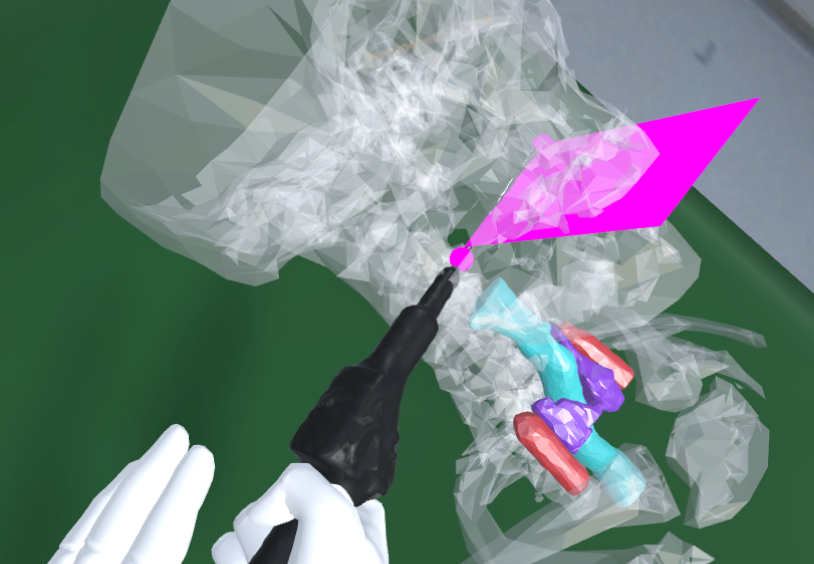
\includegraphics[width=200px]{images/implementation/features/procedures/bonesaw.png}
    \caption{\label{fig::FeatureBoneSaw}Bonesaw Procedure}
\end{figure}

The \textbf{sawing} procedure is performed by picking up the bonesaw.
Touch the controller will show two indications to the user (Figure \ref{fig::FeatureBoneSaw}).
The procedure is performed by first pressing down the trigger button and then letting go of it.
When letting go of the trigger button, a two dimensianal plane is created in the three dimensional space by using four points.
Two of these points are created when pressing down, and the other two when letting go of the trigger button.
A plane is then created with which the user can reproduce the way in which the bonesaw has been moved.
Arbitrary cutting shapes can be created by breaking them down into two-dimensional shapes and performing multiple movements.
\paragraph{Milling}

\begin{figure}[ht]
    \centering
    \includegraphics[width=200px]{images/implementation/features/procedures/piezo.png}
    \caption{\label{fig::FeaturePiezo}Milling procedure. Holding down the trigger button will draw little spheres until the button is released. The resulting object represents the volumetric space which is to be milled.}
\end{figure}

The \textbf{milling} operation is performed by grabbing the piezo instrument.
The indicator for the piezo is at the tip of the instrument, indicating which area will be milled.
While the "perform" button is being held down, little spheres are being drawn at the tip of the instrument \ref{fig::FeaturePiezo}.
When the button is released, the shapes are combined into a single 3D model and added as a project step.
The resulting object represents the volumetric space which has to be milled in the procedure.
The procedure can be reconstructed by "milling" the same 3D space in the virtual operating room.
\begin{figure}[ht!]
    \centering
    \includegraphics[width=\linewidth]{images/implementation/features/procedures/metal_plates_1.png}
    \caption{\label{fig::FeatureMetalPlate} Osteosynthesis Plates Overview}
\end{figure}

The osteosynthesis plates procedure consists of two steps before adding it as a step to the project case.
First, users have to chose which plate to use (Figure \ref{fig::FeatureMetalPlate}).
The user can chose from four reconstruction plates, 29 1.5mm plates and 20 2.0mm plates (Firma Angeben, osteosynthesis plates).
The optimal plates to use vary due to the pathology of the patient and the previously performed procedures.
After selecting the proper plate, a number of indicators will show to the user (Figure \ref{fig::FeatureMetalPlate2}).
In the context of the osteosynthesis plates, these indicators are "control points", with which the user can bend and twist the plates.
Bending and twisting is performed by chosing a control point via hovering them with the users free hand and grabbing them.
Then, the user has to translate and rotate the control point in the desired manner.
\begin{figure}
  \centering
  \begin{minipage}{.5\textwidth}
    \centering
    \includegraphics[width=0.95\linewidth]{images/implementation/features/procedures/metal_plates_2.png}
  \end{minipage}%
  \begin{minipage}{.5\textwidth}
    \centering
    \includegraphics[width=0.95\linewidth]{images/implementation/features/procedures/metal_plates_3.png}
  \end{minipage}
  \caption{\label{fig::FeatureMetalPlate2}Osteosynthesis Plates Modifications. User can translate and rotate "control points" to perform modifications to the plates shape} 
\end{figure}

The user can then observe in which way this has affected the shape of the metal plate and either position the plate on the patient or perform more modifications to the plates via controlpoints.
The correct modification of the metal plates differs quite a lot from real life modifications to the plates.
However even though there is a slight learning curve to it, the modification is consistent and predictable (Figure \ref{fig::FeatureMetalPlate2}).


\begin{figure}[ht!]
    \centering
    \includegraphics[width=\linewidth]{images/implementation/features/procedures/marker.png}
    \caption{\label{fig::FeatureMarker}Marker Procedure}
\end{figure}

The marking procedure is similar to the bonesaw procedure, meaning that rectangular shapes are drawed into the three dimensianal space (Figure \ref{fig::FeatureMarker}).
However, here the created shapes are much thinner.
In contrast to the bonesaw, the virtual hands of the user are also disabled here.
This way, the user can decide to hold the marker in the optimal way.
Since the main objective is marking specific spots on the patient, this is the natural approach.

\chapter{\label{chap::Discussion}Discussion}
At this point, the aforementioned six procedures are implemented in the system.
However, as described in Section \ref{sec::Architecture}, the system is extensible in the regard that new instruments can be implemented.
Currently, the implemented instruments are based on the workflow of OMF surgeons of the UHA: Users can perform drilling, hammer and chisel, bonesaw and milling operations.
Additionally, users can place markings and osteosynthesis plates on the virtual patient.
\\ To perform procedures, a project case has to be loaded first, as described in Section \ref{sec::GraphicalUserInterface}.
In the sense of SteamVRs interaction system described in Section \ref{sec::Architecture}, for each procedure there is an 'indicate' action when the user touches the 'perform' button, as well as an 'perform' action when the user presses the button all the way.
This way, users get a visual feedback when they are about to perform a procedure, as well as having visual indications of where the procedure will start (i.e. tip of the surgical instrument).
After described each procedure individually, how the procedures come together to create the steps for a procedure will be shortly desctribed.
\\ Each procedure will add a step to the project case.
In the sense of the VR-AR-based workflow described in Section \ref{sec::Workflow}, project cases can then be loaded into both parts of the workflow.
The steps are added to the hierarchy of the patient's 3D model and are identified as a step by name.
Through using this kind of approach, extensibility is guaranteed as each new instrument simply has to add some kind of geometry as a step to the project case (Requirements \ref{req::N8}, \ref{req::F3.7}).
It follows that any kind of procedure can then be imported into the AR workflow, even without touching the application.
\\ When a procedure is performed, users get voice feedback confirming that a step has been added to the project case.
Users can also navigate the project cases steps by using the VUIs commands, so that navigation through the steps of the procedure can be done while holding surgical instruments (Requirements \ref{req::N1}, \ref{req::F3.7}).
\\ For some of the surgical instruments, the user representation of the hand will be shown, for others not.
When a surgical instrument has this feature implemented, it is guaranteed that the instrument will always be grabbed and positioned in the same position on the hand, meaning the handgrip will always be the same.
However, in some cases, f.e. sawing with the bonesaw, this feature would prevent users from switching the handgrip of the surgical instrument. 
Therefore, for some instruments, this feature was removed.
Users will not see their virtual hands on the surgical instrument, but can chose to hold it however they want.
The virtual hands will be hidden while holding the instrument, however the instrument still represents the users hand position.
This way, the handgrip of the instrument can be adapted as users see fit.
The decision, on which was decided if hands should be hidden when grabbing an instrument, was made by a trial and error approach with the help of a physician's opinion on whether this features was useful.
The procedure specific implementation will be thoroughly described in the following.

\paragraph{Drilling}

The \textbf{drilling} operation is performed by first picking up the drill handle from the instrument tray via the grabbing action (Figure \ref{fig::FeatureDrillingAttachments}).
Since drills are typically held in a number of different ways, the handgrip of the drill handle is adjustable.
Therefore, the virtual hand will not be displayed while holding the drill.
The instrument tray is located next to the operating table, where the patient's model will initially be positioned.
The drill handle initially has no attachment; users have to attach a drill bit first.

\begin{figure}[ht]
    \centering
    \includegraphics[width=200px]{images/implementation/features/procedures/drilling_attachment.png}
    \caption{\label{fig::FeatureDrillingAttachments}Process of attaching drill bit to the drill handle. With the right hand, the user performs the indicate action by touching 
    the respective button. With the other hand, the bit is picked up by grabbing it and moved into the pink sphere to attach the attachment.}
\end{figure}

In total, there are fifteen bits which can be used as an attachment for the drilling procedure.
Bits are modeled after their real counterparts in UHA.
They differ in size, length and width.
A visual signal is shown to the user while the indicate action is performed on the hand holding the drill handle.
By moving a drill bit to the visual indicator, the bit is attached to the handle (Figure \ref{fig::FeatureDrillingAttachments}).
Swapping out bits is performed by simply moving another bit into the indicator.
To perform the procedure, the drill handle must have a bit attached. 

\begin{figure}[ht]
    \centering
    \includegraphics[width=200px]{images/implementation/features/procedures/drilling.png}
    \caption{\label{fig::FeatureDrilling}Drilling procedure. The pink object represents the last performed step, which was performed using the currently selected tool by pressing 
    the respective button all the way.}
\end{figure}

By triggering the perform action of the hand holding the drill, a copy of the currently attached drill bit is created and added to the project case. 
This copy has a different material, i.e. a pink material, to indicate that it is part of the project case (Figure \ref{fig::FeatureDrilling}).
Additionally, textual information about the currently attached drill bit will be stored in the project case, so that the exact procedure can be reproduced later (Requirements \ref{req::N3}, \ref{req::N5}).
The drill bit will not be removed on performing a procedure, so that multiple drilling steps can be performed consecutively.
When the drill is no longer needed, it can either be placed back on the instrument tray or the operating table for quick access.
Note that any instrument, excluding the osteosynthesis plates described later, can be placed anywhere in the OT.
\paragraph{Chiseling}

The \textbf{chiseling} procedure has two parts to it.
First, with one hand a chisel has to be chosen.
Users have a choice between a small, medium, large and extra large chisel to perform the procedure.
With the other hand, users then have to pick up the hammer.
Since this procedure requires users to hold two surgical instruments at the same time, this procedure can get cumbersome.
However, users can easily avoid this by placing the instruments on the operating table in the middle of the OT and repositioning afterwards (Figure \ref{fig::ChiselPrepare}).

\begin{figure}[ht]
    \centering
    \includegraphics[width=\linewidth]{images/implementation/features/procedures/chisel_prepare.png}
    \caption{\label{fig::ChiselPrepare}The user prepares for the chiseling procedure by placing the instruments on the OT where the patient is located.
    indicators with the hammer in the other hand to perform the procedure.}
\end{figure}

When users have the perfect viewpoint, they can take up both instruments once again and start the procedure.
By pressing the indicate button on the hand where the chisel is located, rectangular indications at the top and bottom end of the chisel are shown to the user.
While these indications are active, the user has to perform a hammering motion with the hand holding the hammer.

\begin{figure}[ht]
    \centering
    \begin{minipage}{.5\textwidth}
      \centering
      \includegraphics[width=0.99\linewidth]{images/implementation/features/procedures/chisel_1.png}
    \end{minipage}%
    \begin{minipage}{.5\textwidth}
      \centering
      \includegraphics[width=0.99\linewidth]{images/implementation/features/procedures/chisel_2.png}
    \end{minipage}
    \caption{\label{fig::ChiselProcedure}Process of the chiseling procedure. Left: The users uses the indicate action with his left hand in preparation for the procedure. Right: After hammering on the indication on the chisel, the procedure has been performed and a step is generated.}
\end{figure}

When they hit the rectangular indicators located on the chisel, the chiseling procedure step is added to the project case in form of a modified copy of the hold chisel (Figure \ref{fig::ChiselProcedure}).
Here, information about the performed step is also included in the form of chisel size used for the procedure. 
\paragraph{Sawing}

\begin{figure}[ht]
    \centering
    \includegraphics[width=200px]{images/implementation/features/procedures/bonesaw.png}
    \caption{\label{fig::FeatureBoneSaw}Bonesaw Procedure}
\end{figure}

The \textbf{sawing} procedure is performed by picking up the bonesaw.
Touch the controller will show two indications to the user (Figure \ref{fig::FeatureBoneSaw}).
The procedure is performed by first pressing down the trigger button and then letting go of it.
When letting go of the trigger button, a two dimensianal plane is created in the three dimensional space by using four points.
Two of these points are created when pressing down, and the other two when letting go of the trigger button.
A plane is then created with which the user can reproduce the way in which the bonesaw has been moved.
Arbitrary cutting shapes can be created by breaking them down into two-dimensional shapes and performing multiple movements.
\paragraph{Milling}

\begin{figure}[ht]
    \centering
    \includegraphics[width=200px]{images/implementation/features/procedures/piezo.png}
    \caption{\label{fig::FeaturePiezo}Milling procedure. Holding down the trigger button will draw little spheres until the button is released. The resulting object represents the volumetric space which is to be milled.}
\end{figure}

The \textbf{milling} operation is performed by grabbing the piezo instrument.
The indicator for the piezo is at the tip of the instrument, indicating which area will be milled.
While the "perform" button is being held down, little spheres are being drawn at the tip of the instrument \ref{fig::FeaturePiezo}.
When the button is released, the shapes are combined into a single 3D model and added as a project step.
The resulting object represents the volumetric space which has to be milled in the procedure.
The procedure can be reconstructed by "milling" the same 3D space in the virtual operating room.
\begin{figure}[ht!]
    \centering
    \includegraphics[width=\linewidth]{images/implementation/features/procedures/metal_plates_1.png}
    \caption{\label{fig::FeatureMetalPlate} Osteosynthesis Plates Overview}
\end{figure}

The osteosynthesis plates procedure consists of two steps before adding it as a step to the project case.
First, users have to chose which plate to use (Figure \ref{fig::FeatureMetalPlate}).
The user can chose from four reconstruction plates, 29 1.5mm plates and 20 2.0mm plates (Firma Angeben, osteosynthesis plates).
The optimal plates to use vary due to the pathology of the patient and the previously performed procedures.
After selecting the proper plate, a number of indicators will show to the user (Figure \ref{fig::FeatureMetalPlate2}).
In the context of the osteosynthesis plates, these indicators are "control points", with which the user can bend and twist the plates.
Bending and twisting is performed by chosing a control point via hovering them with the users free hand and grabbing them.
Then, the user has to translate and rotate the control point in the desired manner.
\begin{figure}
  \centering
  \begin{minipage}{.5\textwidth}
    \centering
    \includegraphics[width=0.95\linewidth]{images/implementation/features/procedures/metal_plates_2.png}
  \end{minipage}%
  \begin{minipage}{.5\textwidth}
    \centering
    \includegraphics[width=0.95\linewidth]{images/implementation/features/procedures/metal_plates_3.png}
  \end{minipage}
  \caption{\label{fig::FeatureMetalPlate2}Osteosynthesis Plates Modifications. User can translate and rotate "control points" to perform modifications to the plates shape} 
\end{figure}

The user can then observe in which way this has affected the shape of the metal plate and either position the plate on the patient or perform more modifications to the plates via controlpoints.
The correct modification of the metal plates differs quite a lot from real life modifications to the plates.
However even though there is a slight learning curve to it, the modification is consistent and predictable (Figure \ref{fig::FeatureMetalPlate2}).


\begin{figure}[ht!]
    \centering
    \includegraphics[width=\linewidth]{images/implementation/features/procedures/marker.png}
    \caption{\label{fig::FeatureMarker}Marker Procedure}
\end{figure}

The marking procedure is similar to the bonesaw procedure, meaning that rectangular shapes are drawed into the three dimensianal space (Figure \ref{fig::FeatureMarker}).
However, here the created shapes are much thinner.
In contrast to the bonesaw, the virtual hands of the user are also disabled here.
This way, the user can decide to hold the marker in the optimal way.
Since the main objective is marking specific spots on the patient, this is the natural approach.

\chapter{\label{chap::Conclusion}Conclusion}
At this point, the aforementioned six procedures are implemented in the system.
However, as described in Section \ref{sec::Architecture}, the system is extensible in the regard that new instruments can be implemented.
Currently, the implemented instruments are based on the workflow of OMF surgeons of the UHA: Users can perform drilling, hammer and chisel, bonesaw and milling operations.
Additionally, users can place markings and osteosynthesis plates on the virtual patient.
\\ To perform procedures, a project case has to be loaded first, as described in Section \ref{sec::GraphicalUserInterface}.
In the sense of SteamVRs interaction system described in Section \ref{sec::Architecture}, for each procedure there is an 'indicate' action when the user touches the 'perform' button, as well as an 'perform' action when the user presses the button all the way.
This way, users get a visual feedback when they are about to perform a procedure, as well as having visual indications of where the procedure will start (i.e. tip of the surgical instrument).
After described each procedure individually, how the procedures come together to create the steps for a procedure will be shortly desctribed.
\\ Each procedure will add a step to the project case.
In the sense of the VR-AR-based workflow described in Section \ref{sec::Workflow}, project cases can then be loaded into both parts of the workflow.
The steps are added to the hierarchy of the patient's 3D model and are identified as a step by name.
Through using this kind of approach, extensibility is guaranteed as each new instrument simply has to add some kind of geometry as a step to the project case (Requirements \ref{req::N8}, \ref{req::F3.7}).
It follows that any kind of procedure can then be imported into the AR workflow, even without touching the application.
\\ When a procedure is performed, users get voice feedback confirming that a step has been added to the project case.
Users can also navigate the project cases steps by using the VUIs commands, so that navigation through the steps of the procedure can be done while holding surgical instruments (Requirements \ref{req::N1}, \ref{req::F3.7}).
\\ For some of the surgical instruments, the user representation of the hand will be shown, for others not.
When a surgical instrument has this feature implemented, it is guaranteed that the instrument will always be grabbed and positioned in the same position on the hand, meaning the handgrip will always be the same.
However, in some cases, f.e. sawing with the bonesaw, this feature would prevent users from switching the handgrip of the surgical instrument. 
Therefore, for some instruments, this feature was removed.
Users will not see their virtual hands on the surgical instrument, but can chose to hold it however they want.
The virtual hands will be hidden while holding the instrument, however the instrument still represents the users hand position.
This way, the handgrip of the instrument can be adapted as users see fit.
The decision, on which was decided if hands should be hidden when grabbing an instrument, was made by a trial and error approach with the help of a physician's opinion on whether this features was useful.
The procedure specific implementation will be thoroughly described in the following.

\paragraph{Drilling}

The \textbf{drilling} operation is performed by first picking up the drill handle from the instrument tray via the grabbing action (Figure \ref{fig::FeatureDrillingAttachments}).
Since drills are typically held in a number of different ways, the handgrip of the drill handle is adjustable.
Therefore, the virtual hand will not be displayed while holding the drill.
The instrument tray is located next to the operating table, where the patient's model will initially be positioned.
The drill handle initially has no attachment; users have to attach a drill bit first.

\begin{figure}[ht]
    \centering
    \includegraphics[width=200px]{images/implementation/features/procedures/drilling_attachment.png}
    \caption{\label{fig::FeatureDrillingAttachments}Process of attaching drill bit to the drill handle. With the right hand, the user performs the indicate action by touching 
    the respective button. With the other hand, the bit is picked up by grabbing it and moved into the pink sphere to attach the attachment.}
\end{figure}

In total, there are fifteen bits which can be used as an attachment for the drilling procedure.
Bits are modeled after their real counterparts in UHA.
They differ in size, length and width.
A visual signal is shown to the user while the indicate action is performed on the hand holding the drill handle.
By moving a drill bit to the visual indicator, the bit is attached to the handle (Figure \ref{fig::FeatureDrillingAttachments}).
Swapping out bits is performed by simply moving another bit into the indicator.
To perform the procedure, the drill handle must have a bit attached. 

\begin{figure}[ht]
    \centering
    \includegraphics[width=200px]{images/implementation/features/procedures/drilling.png}
    \caption{\label{fig::FeatureDrilling}Drilling procedure. The pink object represents the last performed step, which was performed using the currently selected tool by pressing 
    the respective button all the way.}
\end{figure}

By triggering the perform action of the hand holding the drill, a copy of the currently attached drill bit is created and added to the project case. 
This copy has a different material, i.e. a pink material, to indicate that it is part of the project case (Figure \ref{fig::FeatureDrilling}).
Additionally, textual information about the currently attached drill bit will be stored in the project case, so that the exact procedure can be reproduced later (Requirements \ref{req::N3}, \ref{req::N5}).
The drill bit will not be removed on performing a procedure, so that multiple drilling steps can be performed consecutively.
When the drill is no longer needed, it can either be placed back on the instrument tray or the operating table for quick access.
Note that any instrument, excluding the osteosynthesis plates described later, can be placed anywhere in the OT.
\paragraph{Chiseling}

The \textbf{chiseling} procedure has two parts to it.
First, with one hand a chisel has to be chosen.
Users have a choice between a small, medium, large and extra large chisel to perform the procedure.
With the other hand, users then have to pick up the hammer.
Since this procedure requires users to hold two surgical instruments at the same time, this procedure can get cumbersome.
However, users can easily avoid this by placing the instruments on the operating table in the middle of the OT and repositioning afterwards (Figure \ref{fig::ChiselPrepare}).

\begin{figure}[ht]
    \centering
    \includegraphics[width=\linewidth]{images/implementation/features/procedures/chisel_prepare.png}
    \caption{\label{fig::ChiselPrepare}The user prepares for the chiseling procedure by placing the instruments on the OT where the patient is located.
    indicators with the hammer in the other hand to perform the procedure.}
\end{figure}

When users have the perfect viewpoint, they can take up both instruments once again and start the procedure.
By pressing the indicate button on the hand where the chisel is located, rectangular indications at the top and bottom end of the chisel are shown to the user.
While these indications are active, the user has to perform a hammering motion with the hand holding the hammer.

\begin{figure}[ht]
    \centering
    \begin{minipage}{.5\textwidth}
      \centering
      \includegraphics[width=0.99\linewidth]{images/implementation/features/procedures/chisel_1.png}
    \end{minipage}%
    \begin{minipage}{.5\textwidth}
      \centering
      \includegraphics[width=0.99\linewidth]{images/implementation/features/procedures/chisel_2.png}
    \end{minipage}
    \caption{\label{fig::ChiselProcedure}Process of the chiseling procedure. Left: The users uses the indicate action with his left hand in preparation for the procedure. Right: After hammering on the indication on the chisel, the procedure has been performed and a step is generated.}
\end{figure}

When they hit the rectangular indicators located on the chisel, the chiseling procedure step is added to the project case in form of a modified copy of the hold chisel (Figure \ref{fig::ChiselProcedure}).
Here, information about the performed step is also included in the form of chisel size used for the procedure. 
\paragraph{Sawing}

\begin{figure}[ht]
    \centering
    \includegraphics[width=200px]{images/implementation/features/procedures/bonesaw.png}
    \caption{\label{fig::FeatureBoneSaw}Bonesaw Procedure}
\end{figure}

The \textbf{sawing} procedure is performed by picking up the bonesaw.
Touch the controller will show two indications to the user (Figure \ref{fig::FeatureBoneSaw}).
The procedure is performed by first pressing down the trigger button and then letting go of it.
When letting go of the trigger button, a two dimensianal plane is created in the three dimensional space by using four points.
Two of these points are created when pressing down, and the other two when letting go of the trigger button.
A plane is then created with which the user can reproduce the way in which the bonesaw has been moved.
Arbitrary cutting shapes can be created by breaking them down into two-dimensional shapes and performing multiple movements.
\paragraph{Milling}

\begin{figure}[ht]
    \centering
    \includegraphics[width=200px]{images/implementation/features/procedures/piezo.png}
    \caption{\label{fig::FeaturePiezo}Milling procedure. Holding down the trigger button will draw little spheres until the button is released. The resulting object represents the volumetric space which is to be milled.}
\end{figure}

The \textbf{milling} operation is performed by grabbing the piezo instrument.
The indicator for the piezo is at the tip of the instrument, indicating which area will be milled.
While the "perform" button is being held down, little spheres are being drawn at the tip of the instrument \ref{fig::FeaturePiezo}.
When the button is released, the shapes are combined into a single 3D model and added as a project step.
The resulting object represents the volumetric space which has to be milled in the procedure.
The procedure can be reconstructed by "milling" the same 3D space in the virtual operating room.
\begin{figure}[ht!]
    \centering
    \includegraphics[width=\linewidth]{images/implementation/features/procedures/metal_plates_1.png}
    \caption{\label{fig::FeatureMetalPlate} Osteosynthesis Plates Overview}
\end{figure}

The osteosynthesis plates procedure consists of two steps before adding it as a step to the project case.
First, users have to chose which plate to use (Figure \ref{fig::FeatureMetalPlate}).
The user can chose from four reconstruction plates, 29 1.5mm plates and 20 2.0mm plates (Firma Angeben, osteosynthesis plates).
The optimal plates to use vary due to the pathology of the patient and the previously performed procedures.
After selecting the proper plate, a number of indicators will show to the user (Figure \ref{fig::FeatureMetalPlate2}).
In the context of the osteosynthesis plates, these indicators are "control points", with which the user can bend and twist the plates.
Bending and twisting is performed by chosing a control point via hovering them with the users free hand and grabbing them.
Then, the user has to translate and rotate the control point in the desired manner.
\begin{figure}
  \centering
  \begin{minipage}{.5\textwidth}
    \centering
    \includegraphics[width=0.95\linewidth]{images/implementation/features/procedures/metal_plates_2.png}
  \end{minipage}%
  \begin{minipage}{.5\textwidth}
    \centering
    \includegraphics[width=0.95\linewidth]{images/implementation/features/procedures/metal_plates_3.png}
  \end{minipage}
  \caption{\label{fig::FeatureMetalPlate2}Osteosynthesis Plates Modifications. User can translate and rotate "control points" to perform modifications to the plates shape} 
\end{figure}

The user can then observe in which way this has affected the shape of the metal plate and either position the plate on the patient or perform more modifications to the plates via controlpoints.
The correct modification of the metal plates differs quite a lot from real life modifications to the plates.
However even though there is a slight learning curve to it, the modification is consistent and predictable (Figure \ref{fig::FeatureMetalPlate2}).


\begin{figure}[ht!]
    \centering
    \includegraphics[width=\linewidth]{images/implementation/features/procedures/marker.png}
    \caption{\label{fig::FeatureMarker}Marker Procedure}
\end{figure}

The marking procedure is similar to the bonesaw procedure, meaning that rectangular shapes are drawed into the three dimensianal space (Figure \ref{fig::FeatureMarker}).
However, here the created shapes are much thinner.
In contrast to the bonesaw, the virtual hands of the user are also disabled here.
This way, the user can decide to hold the marker in the optimal way.
Since the main objective is marking specific spots on the patient, this is the natural approach.

\printbibliography

\begin{appendices}
    \chapter{\label{appendix::A}A}
\includepdf[pages=-]{appendix/PreStudy.pdf}
\includepdf[pages=-]{appendix/questionnaire.pdf}

\chapter{\label{appendix::B}B}
\begin{table}[h]
    \centering
    \begin{tabular}{llllll}
    \textbf{Participant} & \textbf{Age} & \textbf{Gender} & \textbf{Handed} & \textbf{Vision} & \textbf{Color Blindness} \\
    1             & 32           & m               & right           & normal          & false                     \\
    2             & 34           & m               & left            & normal          & false                     \\
    3             & 28           & m               & right           & normal          & false                     \\
    4             & 32           & m               & right           & corrected       & false                     \\
    5             & 34           & m               & right           & corrected       & false   
    \end{tabular}
    \begin{tabular}{lllll}
    \textbf{Participant} & \textbf{Q6} & \textbf{Q7} & \textbf{Q8} & \textbf{Q9} \\
        1             & b           & a           & c           & c           \\
        2             & b           & b           & b           & b           \\
        3             & b           & b           & b           & b           \\
        4             & b           & c           & c           & c           \\
        5             & c           & b           & c           & c          
    \end{tabular}
    \caption{Informations about the participants gathered in the pre-questionnaire.}
\end{table}
\end{appendices}

\end{document}